%%% The main file. It contains definitions of basic parameters and includes all other parts.
%\pdfminorversion=6
%% Settings for single-side (simplex) printing
% Margins: left 40mm, right 25mm, top and bottom 25mm
% (but beware, LaTeX adds 1in implicitly)
\documentclass[12pt,a4paper]{report}
\setlength\textwidth{145mm}
\setlength\textheight{247mm}
\setlength\oddsidemargin{15mm}
\setlength\evensidemargin{15mm}
\setlength\topmargin{0mm}
\setlength\headsep{0mm}
\setlength\headheight{0mm}
% \openright makes the following text appear on a right-hand page
\let\openright=\clearpage


%% Settings for two-sided (duplex) printing
% \documentclass[12pt,a4paper,twoside,openright]{report}
% \setlength\textwidth{145mm}
% \setlength\textheight{247mm}
% \setlength\oddsidemargin{14.2mm}
% \setlength\evensidemargin{0mm}
% \setlength\topmargin{0mm}
% \setlength\headsep{0mm}
% \setlength\headheight{0mm}
% \let\openright=\cleardoublepage

%% Generate PDF/A-2u
\usepackage[a-2u]{pdfx}

%% Character encoding: usually latin2, cp1250 or utf8:
\usepackage[utf8]{inputenc}

%% Prefer Latin Modern fonts
\usepackage{lmodern}

%% Further useful packages (included in most LaTeX distributions)
\usepackage{amsmath}        % extensions for typesetting of math
\usepackage{amsfonts}       % math fonts
\usepackage{amsthm}         % theorems, definitions, etc.
\usepackage{bbding}         % various symbols (squares, asterisks, scissors, ...)
\usepackage{bm}             % boldface symbols (\bm)
\usepackage{graphicx}       % embedding of pictures
\usepackage{fancyvrb}       % improved verbatim environment
\usepackage{natbib}         % citation style AUTHOR (YEAR), or AUTHOR [NUMBER]
\usepackage[nottoc]{tocbibind} % makes sure that bibliography and the lists
			    % of figures/tables are included in the table
			    % of contents
\usepackage{dcolumn}        % improved alignment of table columns
\usepackage{booktabs}       % improved horizontal lines in tables
\usepackage{paralist}       % improved enumerate and itemize
\usepackage{outlines}       % even better lists
\usepackage{xcolor}         % typesetting in color

\usepackage{subcaption}

\usepackage{csquotes}       % for displayquote

\usepackage{indentfirst}    % alignment of first paragraph in section

\usepackage{rotating}       % rotate figures

% clever references automatically show correct word e.g. Section or Table
\usepackage[noabbrev,capitalize]{cleveref}

\usepackage[toc,acronym]{glossaries}     % for terms and abbreviations
% https://www.overleaf.com/learn/latex/glossaries
% example:
% \acrshort{mt} - MT
% \acrlong{mt} - machine translation
% \acrfull{mt} - MT (machine translation)

% \Gls{latex} - Latex
% \gls{latex} - latex
% \GLS{latex} - LATEX
% \glspl{term} - terms

\makeglossaries

\newglossaryentry{latex}
{
    name=latex,
    description={Is a mark up language specially suited 
    for scientific documents}
}

\newglossaryentry{gradient-descent}
{
    name=gradient descent,
    description={An algorithm of iterative optimization of 
		 differentiable objective function (loss)}
}

\newglossaryentry{stochastic-gradient-descent}
{
    name=stochastic gradient descent,
    description={Method for iterative optimizing an objective function.
		 Differs from \gls{gd} by approximating the gradient
		 on mini-batch of data.}
}

\newglossaryentry{epoch}
{
    name=epoch,
    description={Refers to one pass of full training dataset to the learning 
		 algorightm
		}
}

\newglossaryentry{early-stopping}
{
    name=early stopping,
    description={Regularization technique to avoid model overfit.
		 Usualy consists of stopping the training process
		 when the value of some selected metric on the 
		 validation set is not improved for last number of
		 validation steps.
		}
}

\newglossaryentry{overfitting}
{
    name=overfitting,
    description={
		 Occurs when the model's performance on unseen validation
		 set stops improving while on the training set
		 it still improves.
		}
}

\newglossaryentry{en-to-5}
{
    name=en-to-5,
    description={The dataset created from UN parallel corpus,
	with source sentences in English and target sentences
	in one of following 5 languages: Spanish, French, Russian,
	Arabic and Chinese; described in Section \ref{subsection:en-to-5}
	}
}

\newglossaryentry{en-to-36}
{
    name=en-to-36,
    description={The dataset with source sentences in English
	and target sentences in 36 languages, described
	in Section \ref{subsection:en-to-36}
	}
}

\newacronym{mt}{MT}{machine translation}
\newacronym{smt}{SMT}{statistical machine translation}
\newacronym{nmt}{NMT}{neural machine translation}
\newacronym{sgd}{SGD}{stochastic gradient descent}
%%% \newacronym{}{}{}
%%% WMT18, WMT19, WMTxx -- annual Workshop on Statistical Machine Translation
%%% (year 2018, 2019, 20xx resp.)
\newacronym{rnn}{RNN}{recurrent neural network}
\newacronym{cnn}{CNN}{convolutional neural network}
\newacronym{lstm}{LSTM}{long short-term memory}
% --  (RNN architecture)
\newacronym{gru}{GRU}{gated recurrent unit}
\newacronym{alpac}{ALPAC}{Automatic Language Processing Advisory Committee}
\newacronym{arpa}{ARPA}{Advanced Research Projects Agency}
\newacronym{bleu}{BLEU}{bilingual evaluation understudy}
%--  (method of automatic MT evaluation)
%%% \newacronym{}{}{}


%%% Basic information on the thesis

% Thesis title in English (exactly as in the formal assignment)
\def\ThesisTitle{Multi-Target Machine Translation}

% Author of the thesis
\def\ThesisAuthor{Bohdan Ihnatchenko}

% Year when the thesis is submitted
\def\YearSubmitted{2020}

% Name of the department or institute, where the work was officially assigned
% (according to the Organizational Structure of MFF UK in English,
% or a full name of a department outside MFF)
\def\Department{Institute of Formal and Applied Linguistics}

% Is it a department (katedra), or an institute (ústav)?
\def\DeptType{Institute}

% Thesis supervisor: name, surname and titles
\def\Supervisor{doc. RNDr. Bojar Ondřej, Ph.D.}

% Supervisor's department (again according to Organizational structure of MFF)
\def\SupervisorsDepartment{Institute of Formal and Applied Linguistics}

% Study programme and specialization
\def\StudyProgramme{Computer Science}
\def\StudyBranch{Artificial Intelligence}

% An optional dedication: you can thank whomever you wish (your supervisor,
% consultant, a person who lent the software, etc.)
\def\Dedication{%
}

% Abstract (recommended length around 80-200 words; this is not a copy of your thesis assignment!)
\def\Abstract{%

In international and highly-multilingual environments,
it often happens, that a talk, a document, or any other
input, needs to be translated into a massive number of other languages.
However, it is not always an option to have a distinct system for each
possible language pair due to the fact that training and operating
such kind of translation systems is computationally demanding.

Combining multiple target languages into one translation model usually
causes a decrease in quality of output for each its translation
direction.
In this thesis, we experiment with combinations of target languages
to see, if a specific grouping of them can lead to better results
than just randomly selecting target languages.

We build upon a recent research on training a multilingual
Transformer model without any change to its architecture:
adding a target language tag to the source sentence.

We trained a large number of bilingual and multilingual
Transformer models and evaluated them on multiple test sets
from different domains.
We found that in most of the cases grouping related
target languages into one model caused a better performance
compared to models with randomly selected languages.
However, we also found that a domain of the test set,
as well as domains of data sampled into the training set,
usually have a more significant effect on improving or
deterioration of multilingual model's translation quality
compared to the bilingual one.

}

% 3 to 5 keywords (recommended), each enclosed in curly braces
\def\Keywords{%
	{Neural machine translation}, {Multi-target MT},
	{linguistic relatedness}
}

%% The hyperref package for clickable links in PDF and also for storing
%% metadata to PDF (including the table of contents).
%% Most settings are pre-set by the pdfx package.
\hypersetup{unicode}
\hypersetup{breaklinks=true}

% Definitions of macros (see description inside)
%%% This file contains definitions of various useful macros and environments %%%
%%% Please add more macros here instead of cluttering other files with them. %%%

%%% Minor tweaks of style

% These macros employ a little dirty trick to convince LaTeX to typeset
% chapter headings sanely, without lots of empty space above them.
% Feel free to ignore.
\makeatletter
\def\@makechapterhead#1{
  {\parindent \z@ \raggedright \normalfont
   \Huge\bfseries \thechapter. #1
   \par\nobreak
   \vskip 20\p@
}}
\def\@makeschapterhead#1{
  {\parindent \z@ \raggedright \normalfont
   \Huge\bfseries #1
   \par\nobreak
   \vskip 20\p@
}}
\makeatother

% This macro defines a chapter, which is not numbered, but is included
% in the table of contents.
\def\chapwithtoc#1{
\chapter*{#1}
\addcontentsline{toc}{chapter}{#1}
}

% Draw black "slugs" whenever a line overflows, so that we can spot it easily.
\overfullrule=1mm

%%% Macros for definitions, theorems, claims, examples, ... (requires amsthm package)

\theoremstyle{plain}
\newtheorem{thm}{Theorem}
\newtheorem{lemma}[thm]{Lemma}
\newtheorem{claim}[thm]{Claim}

\theoremstyle{plain}
\newtheorem{defn}{Definition}

\theoremstyle{remark}
\newtheorem*{cor}{Corollary}
\newtheorem*{rem}{Remark}
\newtheorem*{example}{Example}

%%% An environment for proofs

\newenvironment{myproof}{
  \par\medskip\noindent
  \textit{Proof}.
}{
\newline
\rightline{$\qedsymbol$}
}

%%% An environment for typesetting of program code and input/output
%%% of programs. (Requires the fancyvrb package -- fancy verbatim.)

\DefineVerbatimEnvironment{code}{Verbatim}{fontsize=\small, frame=single}

%%% The field of all real and natural numbers
\newcommand{\R}{\mathbb{R}}
\newcommand{\N}{\mathbb{N}}

%%% Useful operators for statistics and probability
\DeclareMathOperator{\pr}{\textsf{P}}
\DeclareMathOperator{\E}{\textsf{E}\,}
\DeclareMathOperator{\var}{\textrm{var}}
\DeclareMathOperator{\sd}{\textrm{sd}}

%%% Transposition of a vector/matrix
\newcommand{\T}[1]{#1^\top}

%%% Various math goodies
\newcommand{\goto}{\rightarrow}
\newcommand{\gotop}{\stackrel{P}{\longrightarrow}}
\newcommand{\maon}[1]{o(n^{#1})}
\newcommand{\abs}[1]{\left|{#1}\right|}
\newcommand{\dint}{\int_0^\tau\!\!\int_0^\tau}
\newcommand{\isqr}[1]{\frac{1}{\sqrt{#1}}}

%%% Various table goodies
\newcommand{\pulrad}[1]{\raisebox{1.5ex}[0pt]{#1}}
\newcommand{\mc}[1]{\multicolumn{1}{c}{#1}}

% abstracting away the citation styles
\def\perscite#1{\citet{#1}}   % looks like Novak (2014)
\def\parcite#1{\citep{#1}}    % looks like (Novak, 2014)
\def\inparcite#1{\citealp{#1}}   % to be used in paretheses: Novak, 2014
\def\XXX#1{\textcolor{red}{XXX #1}}
\def\fXXX#1{\textcolor{red}{\footnote{\XXX{#1}}}}
\def\red#1{\textcolor{red}{#1}}
\def\repl#1#2{\textcolor{red}{\sout{#1}}\textcolor{blue}{#2}}
\def\todo#1{\XXX{TODO: #1}}
\def\to{$\rightarrow$}


% Terms and abbreviations
%% https://www.overleaf.com/learn/latex/glossaries
% example:
% \acrshort{mt} - MT
% \acrlong{mt} - machine translation
% \acrfull{mt} - MT (machine translation)

% \Gls{latex} - Latex
% \gls{latex} - latex
% \GLS{latex} - LATEX
% \glspl{term} - terms

\makeglossaries

\newglossaryentry{latex}
{
    name=latex,
    description={Is a mark up language specially suited 
    for scientific documents}
}

\newglossaryentry{gradient-descent}
{
    name=gradient descent,
    description={An algorithm of iterative optimization of 
		 differentiable objective function (loss)}
}

\newglossaryentry{stochastic-gradient-descent}
{
    name=stochastic gradient descent,
    description={Method for iterative optimizing an objective function.
		 Differs from \gls{gd} by approximating the gradient
		 on mini-batch of data.}
}

\newglossaryentry{epoch}
{
    name=epoch,
    description={Refers to one pass of full training dataset to the learning 
		 algorightm
		}
}

\newglossaryentry{early-stopping}
{
    name=early stopping,
    description={Regularization technique to avoid model overfit.
		 Usualy consists of stopping the training process
		 when the value of some selected metric on the 
		 validation set is not improved for last number of
		 validation steps.
		}
}

\newglossaryentry{overfitting}
{
    name=overfitting,
    description={
		 Occurs when the model's performance on unseen validation
		 set stops improving while on the training set
		 it still improves.
		}
}

\newglossaryentry{en-to-5}
{
    name=en-to-5,
    description={The dataset created from UN parallel corpus,
	with source sentences in English and target sentences
	in one of following 5 languages: Spanish, French, Russian,
	Arabic and Chinese; described in Section \ref{subsection:en-to-5}
	}
}

\newglossaryentry{en-to-36}
{
    name=en-to-36,
    description={The dataset with source sentences in English
	and target sentences in 36 languages, described
	in Section \ref{subsection:en-to-36}
	}
}

\newacronym{mt}{MT}{machine translation}
\newacronym{smt}{SMT}{statistical machine translation}
\newacronym{nmt}{NMT}{neural machine translation}
\newacronym{sgd}{SGD}{stochastic gradient descent}
%%% \newacronym{}{}{}
%%% WMT18, WMT19, WMTxx -- annual Workshop on Statistical Machine Translation
%%% (year 2018, 2019, 20xx resp.)
\newacronym{rnn}{RNN}{recurrent neural network}
\newacronym{cnn}{CNN}{convolutional neural network}
\newacronym{lstm}{LSTM}{long short-term memory}
% --  (RNN architecture)
\newacronym{gru}{GRU}{gated recurrent unit}
\newacronym{alpac}{ALPAC}{Automatic Language Processing Advisory Committee}
\newacronym{arpa}{ARPA}{Advanced Research Projects Agency}
\newacronym{bleu}{BLEU}{bilingual evaluation understudy}
%--  (method of automatic MT evaluation)
%%% \newacronym{}{}{}


% Title page and various mandatory informational pages
\begin{document}
%%% Title page of the thesis and other mandatory pages

%%% Title page of the thesis

\pagestyle{empty}
\hypersetup{pageanchor=false}
\begin{center}

\centerline{\mbox{
\includegraphics[width=166mm]{../img/logo-en.pdf}}}

\vspace{-8mm}
\vfill

{\bf\Large MASTER THESIS}

\vfill

{\LARGE\ThesisAuthor}

\vspace{15mm}

{\LARGE\bfseries\ThesisTitle}

\vfill

\Department

\vfill

{
\centerline{\vbox{\halign{\hbox to 0.45\hsize{\hfil #}&\hskip 0.5em\parbox[t]{0.45\hsize}{\raggedright #}\cr
Supervisor of the master thesis:&\Supervisor \cr
\noalign{\vspace{2mm}}
Study programme:&\StudyProgramme \cr
\noalign{\vspace{2mm}}
Study branch:&\StudyBranch \cr
}}}}

\vfill

% Zde doplňte rok
Prague \YearSubmitted

\end{center}

\newpage

%%% Here should be a bound sheet included -- a signed copy of the "master
%%% thesis assignment". This assignment is NOT a part of the electronic
%%% version of the thesis. DO NOT SCAN.
This is not a~part of the electronic version of the thesis, do not scan!

%%% A page with a solemn declaration to the master thesis

\openright
\hypersetup{pageanchor=true}
\pagestyle{plain}
\pagenumbering{roman}
\vglue 0pt plus 1fill

\noindent
I declare that I carried out this master thesis independently, and only with the cited
sources, literature and other professional sources. It has not been used to obtain another
or the same degree.

\medskip\noindent
I understand that my work relates to the rights and obligations under the Act No.~121/2000 Sb.,
the Copyright Act, as amended, in particular the fact that the Charles
University has the right to conclude a license agreement on the use of this
work as a school work pursuant to Section 60 subsection 1 of the Copyright~Act.

\vspace{10mm}

\hbox{\hbox to 0.5\hsize{%
In \hbox to 6em{\dotfill} date \hbox to 6em{\dotfill}
\hss}\hbox to 0.5\hsize{\dotfill\quad}}
\smallskip
\hbox{\hbox to 0.5\hsize{}\hbox to 0.5\hsize{\hfil Author's signature\hfil}}

\vspace{20mm}
\newpage

%%% Dedication

\openright

\noindent
\Dedication

\newpage

%%% Mandatory information page of the thesis

\openright

\vbox to 0.5\vsize{
\setlength\parindent{0mm}
\setlength\parskip{5mm}

Title:
\ThesisTitle

Author:
\ThesisAuthor

\DeptType:
\Department

Supervisor:
\Supervisor, \SupervisorsDepartment

Abstract:
\Abstract

Keywords:
\Keywords

\vss}

\newpage

\openright
\pagestyle{plain}
\pagenumbering{arabic}
\setcounter{page}{1}


%%% A page with automatically generated table of contents of the master thesis
\tableofcontents

%%% Each chapter is kept in a separate file
\chapter*{Introduction}
\addcontentsline{toc}{chapter}{Introduction}
With increasing availability of computational resources and enormous amount
of publicly available corpora it is now possible to obtain
a \acrfull{mt} system, which produces translations of acceptable quality.
But in the use cases similar to conferences, where one speech is translated
into multiple target languages, the same amount of models needs to be deployed.
Another option is to use multilingual \acrshort{mt} system for all needed languages together,
which may lead to a decreased quality of translations. \par

The aim of this master thesis is to explore whether the relatedness of target languages in multitarget models could soften the translation quality decrease, caused by adding more and more languages into the mix.


The presented work consists of five chapters:
\begin{itemize}
    \item In the first chapter, we introduce the theoretical background for this thesis.

 \item In the second chapter, we describe the setup for the experiments.
First, we specify the questions to be answered and propose the experimets to do that:
bilingual systems, multilingual systems with unrelated target languages, and then
multilingual systems with related target languages.
Then, we describe the data that was used, its preprocessing and sampling.
After that, we describe the training pipeline and the experiment monitoring tools.

 \item In the third section, we present some selected results that were received after training
bilingual models and multilingual models with unrelated target languages.

 \item In the fourth section, we present the most relevant results from the main experiment --
multilingual models with related targets.

 \item In the discussion section, we present the result, received during a set of experiments, described in Chapter 3 and Chapter 4.

\end{itemize}
\chapter{Background}

\section{\todo{History of machine translation}}

\XXX{is it ok to quote the whole paragraph with short history? e.g. \cite{Han2016}}

\section{\todo{Transformer model}}

Introduced in \perscite{vaswani-2017-transformer} Transformer model is used as a base
for numerous state-of-the-art systems as can be seen for example in 
WMT18 \parcite{bojar-etal-2018-findings} and
WMT19 \parcite{barrault-EtAl:2019:WMT} results.

Prior to invention of the \textit{Transformer} model, \acrfull{rnn} and \acrfull{cnn}
architectures were used
to encode source side of the sentence pair and to decode it into the target sentence.
Various window lengths in \acrshort{cnn} architectures allowed to capture long range relations
as well as short range ones; still the range was limited by the maximum window length.
In \acrshort{rnn}-like architectures \acrfull{lstm} and \acrfull{gru} cells were used,
as their structure allowed to pass the internal state on longer distances
due to selective forgetting.

\textit{Transformer} model uses \textit{self attention} mechanism to encode contextual
information in each word position. \textit{Position encoding} allows passing the position
information without explisit sequential connections as in \acrshort{rnn}.
As was stated by \textit{Transformer}'s authors, there are three main points why
self-attention mechanism should be preferred:
\begin{itemize}
  \item total computational complexity per layer;
  \item the amount of computation that can be parallelized;
  \item the path length between long-range dependencies in the network.
\end{itemize}

\begin{table}
\centering
\begin{tabular}{l|ccc}
\toprule
Layer type        &   Complexity             &  Sequential & Maximum        \\
                  &   per layer              &  operations & path length    \\
\midrule
Self-Attention    & $O(n^2 \cdot d)$         & $O(1)$      & $O(1)$         \\
Recurrent         & $O(n \cdot d^2)$         & $O(n)$      & $O(n)$         \\
Convolutional     & $O(k \cdot n \cdot d^2)$ & $O(1)$      & $O(log_k (n))$ \\
Self-Attention (restricted) & $O(r \cdot n \cdot d)$       & $O(1)$ & $O(n/r)$  \\
\bottomrule
\end{tabular}
\mycaption{Maximum path lengths, per-layer complexity and minimum number of sequential operations for different layer types} {
	n is the sequence length, 
	d is the representation dimension, 
	k is the kernel size of convolutions and 
	r the size of the neighborhood in restricted self-attention.
}
\label{tab:layer_complexity_comp}
\end{table}


\begin{figure}[h]
	\centering
	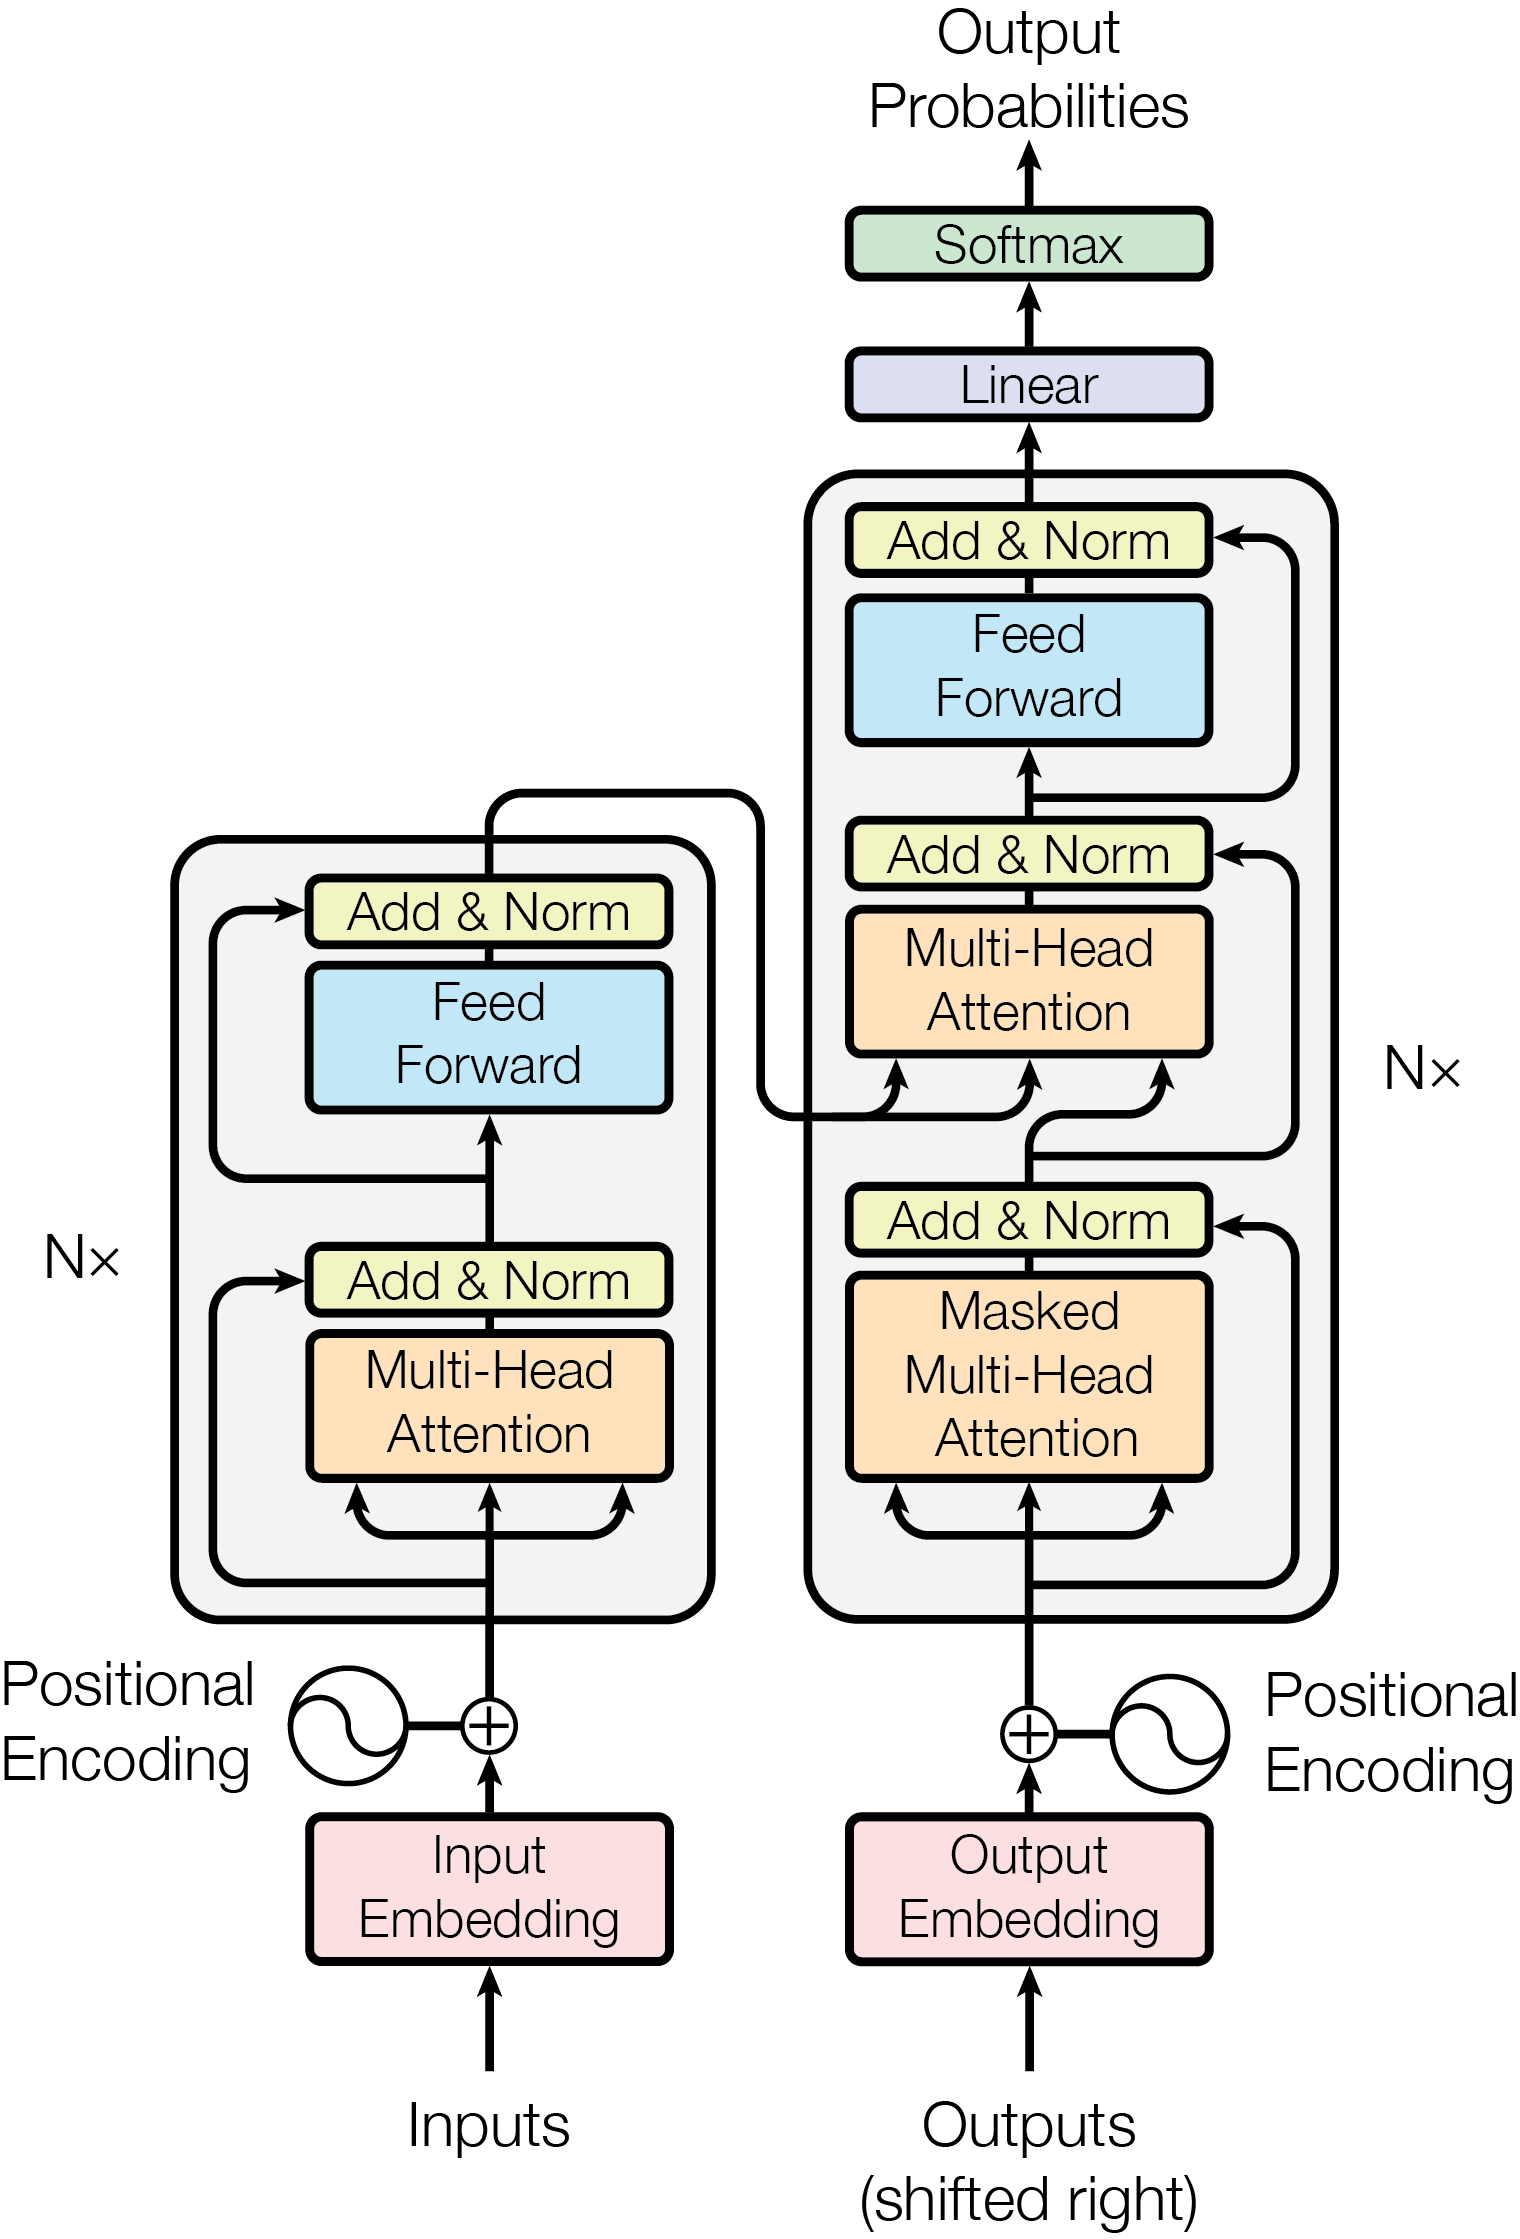
\includegraphics[width=0.9\columnwidth]{../img/transformer_architecture.png}
	\mycaption{Transformer model architecture} {}
	\label{fig:transformer_architecture}
\end{figure}


\section{\todo{Translation evaluation}}

\subsection{History}

In 1966 first machine translation evaluation methods were proposed
by the \acrfull{alpac}.
The proposed metrics were "intelligibility" and "fidelity"\citep[p~67]{Translation1966}.
Metrics were considered independent and the evaluation was meant to be conducted
by two independent groups of raters.
\textit{Intelligibility} was measured without reference to the original by
group of raters fluent in target language and not familiar with the source language.
The raters were comparing the "informativeness" of evaluated translation with carefully
prepared reference translation. The metric scale was from 1 (hopelessly unintelligible)
to 9 (perfectly clear and intelligible).
\textit{Fidelity} to the sense of the original text was measured by another group of raters,
which were native speakers of the target language and highly proficient in the source language.
It was measured on a scale of 0-9 and showed how much additional information was added in
the evaluated translation comparing to the reference translation.

\acrfull{arpa}
\todo{from White 1999 and Church 1993}
comprehension evaluation, quality panel evaluation, and evaluation based on adequacy and fluency

Automatic evaluation

- Metric should correlate with human judgments;

- Works with texts of different domains

- Banerjee et al. (2005) correlation, sensitivity, consistency, reliability and generality.

\subsection{\todo{\acrshort{bleu} - bilingual evaluation understudy}}

In \cite{Papineni02bleu} was introduced a nowel method of automatic machine
translation evaluation - \acrfull{bleu}.
Its advantages are high speed and low cost of evaluation,
language independence and high correlation with judgements
of highly skilled human raters evaluations.

Shortly, \acrshort{bleu} score incorporates modified n-gram precision scores
corrected by brevity penalty,
which ensures the produced translation lenght is close to the reference one.
\acrshort{bleu} score is computed for the whole test corpus.

\subsubsection*{Modified \textit{n}-gram precision score}

The main element of the metric is the \textit{precision} measure.
To compute precision, the number of candidation translatin words (unigrams) that are present in
any reference translation is divided by the total number of words in the candidate translation.
This approach leads to overrating candidate translation which consist of only one or couple of
words that occur in reference translations, as can be seen in the expample below.

Intuitively, after a word from the reference translation has occured it should not be considered
in the calculation anymore.
This intuition is formalized as the \textit{modified unigram precision}.
It is computed in the following way: first, the maximum number of occurances of a word in any
reference translation is counted; then the total count of every candidate word is replaced by the
maximum reference count, added up and divided by the initial total number of candidate words.
As a result, the sentence which may receive high precision score will receive more realistic evaluation
measured by modified precision score, as can be seen in the example below.\\

Candidate: \underline{of} \underline{of} \underline{of} of of of of of of of

Reference: London is the capital \underline{of} England and \underline{of} the United Kingdom
\underline{of} Great Britain and Northern Ireland.

Precision: 1

Modified unigram precision: 3/10
\\
Similarly is computed modified \textit{n}-gram precision score for any \textit{n}, but \textit{n}-gram
counts are collected instead.

\subsubsection*{\todo{Sentence length}}

\subsubsection*{\todo{The formula}}


\section{Multi-target machine translation}
\label{section:multitarget_mt}

\subsection{Multi-lingual machine translation}

With constant improvement of neural \acrshort{mt} systems performance researchers started to
experiment with incorporating multiple source and/or target languages into one model,
and the results are promising: having L1\to{}L2 and L2\to{}L3 non-parallel
corpora makes possible to train a model that can produce L1\to{}L3 tranlsation
of decent quality; having high-resource L1 and low-resource L2 from the same language
group helps increase Source\to{}L2 trainslation quality with pretraining on
Source\to{}L1 data.
In general, in some situations using more target and/or source languages in one translation
model may not only unsignificantly decrease its performance but also to improve it.

Even if the concept of combining multiple languages into one model and possible outcomes
of such combination may seem intuitive, there exist multiple approaches of how exactly
this might be performed. As for current time, \cite{Dabre2019} categorizes
MNMT (multi-lingual neural machine translation) in the following way
(Figure \ref{fig:mnmt_categorized}):

\textbf{Multivay translation.}
The goal is constructing a single \acrshort{nmt} system for
one-to-many, many-to-one or many-to-many
translation using parallel corpora for more than one language pair.

\textbf{Low or Zero-Resource Translation.}
Large amount of parallel texts of high quality is available for most of European
languages. However, it is not true for most of other languages in the world.
Three main directions have been studied these cases.
\textit{Transfer learning}: Transferring translation knowledge from a high-resource language pair
to improve the translation of a low-resource language pair.
\textit{Pivot translation}: Using a high-resource language (usually English) as a pivot to translate
between a language pair.
\textit{Zero-shot translation}: Translating between language pairs without parallel corpora.

\textbf{Multi-Source Translation.} Important documents and internationally popular books have
been translated into many languages. Having the source side represented by multiple languages
may increase translation quality in general or help to remove ambiguities present in one or another
source language (e.g. cases, noun genders, etc.).


\begin{figure}[h]
	\begin{minipage}{0.9\textwidth}
	\centering
	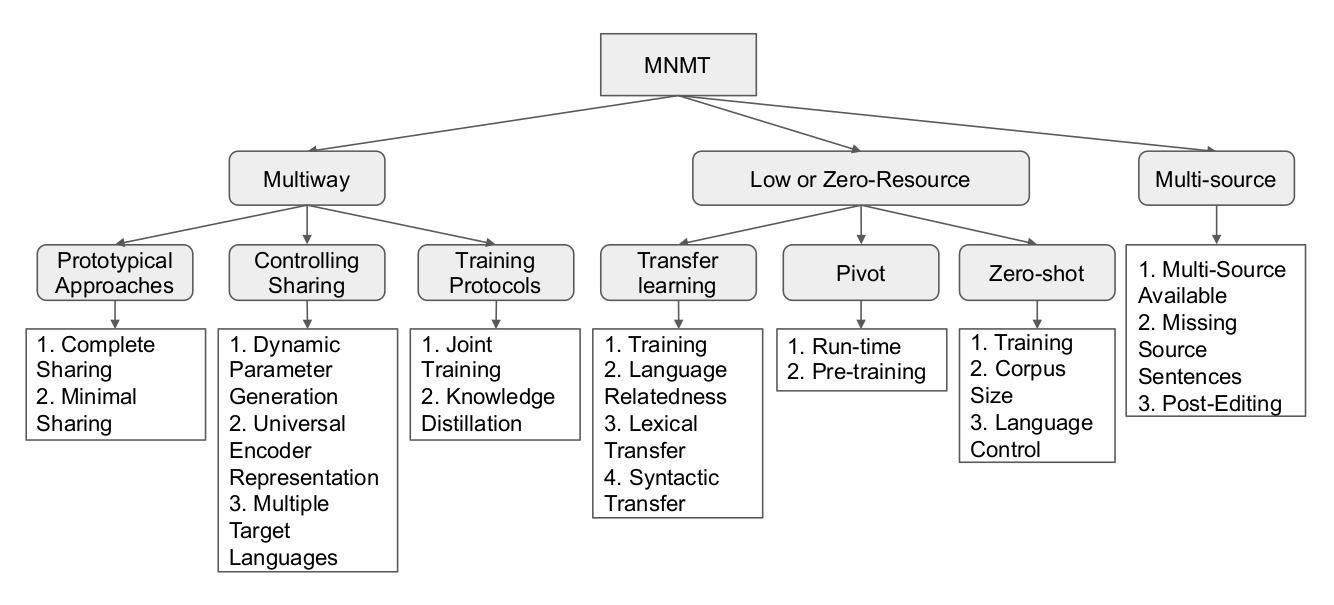
\includegraphics[width=1.0\columnwidth]{../img/dabre_2019_mnmt_categorized.png}
	\end{minipage}\hfill
	\mycaption{%
		MNMT research categorized%
	}{%
		According to resource scenarios and underlying modeling principles.
		By \cite{Dabre2019}
	}
	\label{fig:mnmt_categorized}
\end{figure}


\subsection{Massively multi-lingual machine translation with complete sharing}
\label{section:multitarget_theory}

In \cite{aharoni-etal-2019-massively} models with up to 103 languages were tested.
English centric in-house dataset was used to train En\to{}Any and Any\to{}En multilingual models.
The average number of examples per language pair is 940k:
for 13 out of the 102 pairs there were less than one million examples available.
All languages from 5-to-5 model are present in 25-to-25, same is true for all languages from 25-to-25 with respect to 50-to-50 and so forth.
In all cases they trained large Transformer model with 473.7M parameters.
As can be seen on Table \ref{tab:aharoni-2019-performance-drop}, the quality of translation
is significantly worse when model is trained to translate more languages.
However, it is worth reminding that this many-to-many experiment may have different results due to many-to-one direction present in it.

The decrease of model's performance with adding more target langueges
is clearly shown in \cite{aharoni-etal-2019-massively}.


\begin{table}[h!]
\centering
\begin{tabular}{r|cccc}
\toprule
           & En-Ar & En-Fr & En-Ru & En-Uk \\
\midrule
5-to-5     & \textbf{12.42} & \textbf{37.3} & \textbf{24.86} &         16.48  \\
25-to-25   &         11.77  &         36.79 &         23.24  & \textbf{17.17} \\
50-to-50   &         11.65  &         35.83 &         21.95  &         15.32  \\
75-to-75   &         10.69  &         34.35 &         20.7   &         14.59  \\
103-to-103 &         10.25  &         34.42 &         19.9   &         13.89  \\
\bottomrule
\end{tabular}
\mycaption{\acrshort{bleu} scores for translation in one direction
        (part of Table 7 from \citep{aharoni-etal-2019-massively})
	}{
		Model trained on 5-to-5 English centric dataset
		(English to any and any to English) scores 12.42 \acrshort{bleu} for
		English-Arabic test set. Every language from 5 languages
		of 5-to-5 data set is included into 25-to-25 set, as well
		as every language from 25-to-25 data set is included into
		50-to-50 and so forth.
	}
\label{tab:aharoni-2019-performance-drop}
\end{table}


\begin{figure}[h]
	\begin{minipage}{0.48\textwidth}
	\centering
	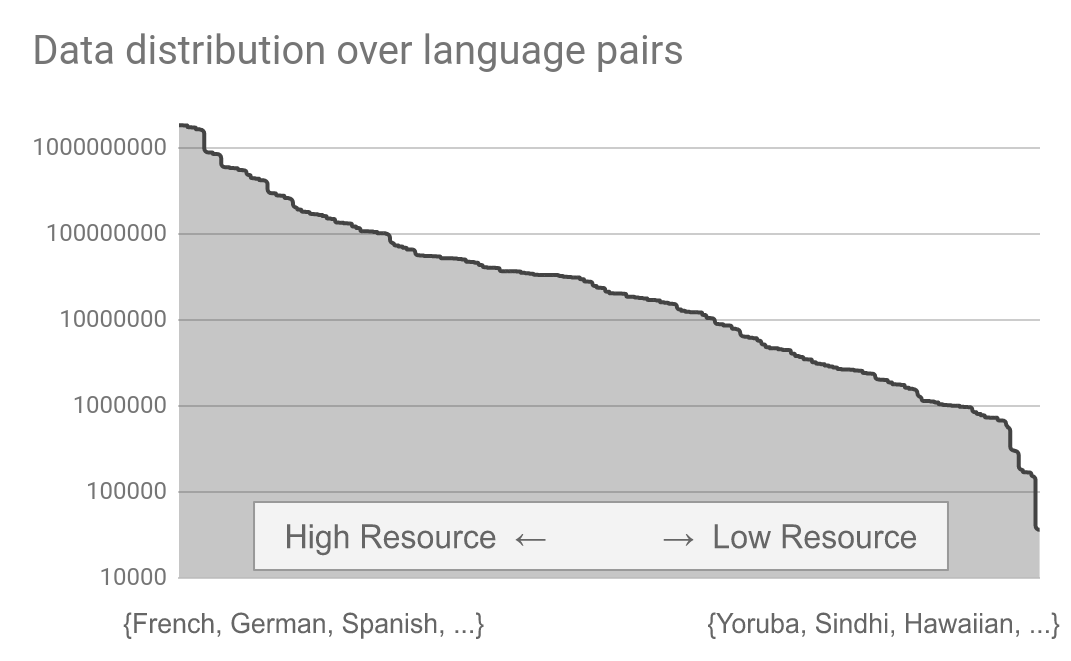
\includegraphics[width=0.9\columnwidth]{../img/arivazhagan-2019-data-distribution.png}
	\end{minipage}\hfill
	%\vspace*{\floatsep}% https://tex.stackexchange.com/q/26521/5764
	\begin{minipage}{0.48\textwidth}
	\centering
	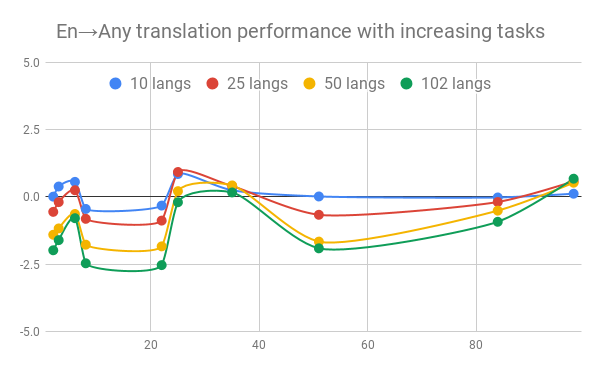
\includegraphics[width=0.9\columnwidth]{../img/arivazhagan-2019-diff-per-n-targets.png}
	\end{minipage}
	\mycaption{
		Tranlsation performance for 102 languages from
		\citet{arivazhagan-2019-mmnmt-in-the-wild}
	}{
		Axis \emph{X} is shared between left and right plot.
		On axis \emph{X} there are languages sorted by amount of training data.
		Left: amount of training data (axis \emph{Y}) for a language.
		Right (best viewed in color): Effect of increasing the number of languages on
		the translation quality. On the axis \emph{X} the languages are sorted the
		same way as on the left plot. The points visualized are 10 languages
		that are present in all setups
		from En $\leftrightarrow$ 10 to En $\leftrightarrow$ 102.
	}
	\label{fig:arivazhagan-2019-diff-per-n-targets}
\end{figure}


\subsection{Conclusion}

In this chapter we introduced theoretical and historical background for this work.
Firstly, we took a short walk through the history of machine translation.
Then we described the most used type of \acrshort{nmt} models --
self-attention \textit{Transformer} model.
After that we went over the history of translation evaluation in general and the most
used method of automatic evaluation -- \acrshort{bleu} -- in particular.
In the end multi-lingual neural machine tranlsation was reviewed with more detailed view into
'complete sharing' scheme.

\chapter{Experiment setup}
\label{chapter:experiment_setup}

In this chapter, we describe the data used for experiments, training setup
and experiments that were run to answer the questions asked in this thesis.

%----------------------------------------------------------------------
\section{\todo{Questions and constraints}}
\label{section:questions_and_constraints}

Constraints:
\begin{displayquote}
	Translation quality for multi-lingual system is better or insignificantly
	worse than for mono-lingual one-to-one tranlsation system.

	Maximum possible target languages are combined in one model.
\end{displayquote}

Questions:
\begin{displayquote}
	How, \emph{on average}, does adding one more randomly selected target language
	to the multitarget model affect its En\to{}De performance?

	How is it different if we add a linguistically similar,
	not a randomly selected language?

	How does adding one more language from the same language family or group 
	\emph{on average} affect translation performance for a selected language
	pair (e.g. En\to{}De)?
\end{displayquote}



%----------------------------------------------------------------------
\section{Experiments}
\label{section:experiments}
\subsection{Starting point}
\label{subsection:starting_point}

The approach described in \cref{section:multitarget_theory} with combining multiple
translation directions into the standart \emph{Transformer} model can be also used to
train just multi-target models, i.e. with one source language and multiple target languages.
The following papers
(\perscite{arivazhagan-2019-mmnmt-in-the-wild}, \perscite{aharoni-etal-2019-massively}),
which further develop the approach, describe and try many different interesting cases.
However, in each setting there is usually only one model of each kind considered.
For example, when in \citet{aharoni-etal-2019-massively} compares 5-to-5,
25-to-25, 50-to-50, etc. models, there is only one 5-to-5 model, one 25-to-25, etc.

To conduct our experiments, we use this approach, but with the following differences:
\begin{itemize}
	\item We fix English as a source language, as we are exploring the multi-target experiments only, .
	\item For every translation direction and every setting we train multiple models.
	E.g. for the \dir{En}{De} translation direction and 1-to-5 setting there are
	couple of \dirmany{En}{De + 4 randomly selected targets} models.
	\item We use only up to 5 target languages in the model because of:
	\begin{itemize}
		\item limited resources;
		\item our selected datasets (which will be described in the next section)
		do not contain more than 5-6 languages of the same language group.
	\end{itemize}
\end{itemize}



\subsection{Proposed experiments}
\label{subsection:proposed_experiments}

% Given the questions and constraints given in \ref{section:questions_and_constraints},
% the variable object in experiments is the data itself. Due to that, the setup similar
% to \cite{johnson-etal-2017-googles} was chosen. 

\subsubsection*{Bilingual \gls{baseline}}

Bilingual models. The purpose is to have a reference point to be able to reason how
does every additional target language affects the model's performance.
\perscite{Siddhant2019} shows that using target language tags results
in the same model efficiency as separately encoding the target.
Therefore, we use target tags in this setting too, so that we can use
the same training pipeline.

\subsubsection*{Multi-lingual baselines (RANDOM)}

Multilingual models with a random set of target languages.
The purpouse is twofold: 
to show \acrshort{bleu} score decrease with increasing number of target languages and
to serve as a baseline for multitarget models with target languages grouped by
in non-random way, e.g. by language group or linguistic similarity.


\subsubsection*{Group by language group (SIMILAR)}

Multilingual models with a set of target languages from the same language group.
Due to shared parts of vocabulary and linguistic properties we expect to
see better results than for multi-lingual baselines.
Ideally the results could be comparable with bilingual baselines.


% \subsubsection*{Group by linguistic similarity}
% 
% From \perscite{siddhant-2020-x-ling-effect} follows that languages' script
% and similarly the amount of shared vocabulary is not so important
% for XX\to{}En translation direction.
% Example with Serbian and Croatian, with the same vocabulary but
% in different scripts.


%----------------------------------------------------------------------
\section{Dataset(s)}
\label{section:datasets}


\subsection{\edit{English to 36 languages}}
\label{subsection:en-to-36}

To observe effects of linguistic similarity of target languages,
it is important to examine enough possible variations of those.
The OPUS dataset (\cite{TIEDEMANN12.463}) is an open and free collection of texts
that covers more than 90 languages with data from several
domains.\footnote{Available at \url{http://opus.nlpl.eu/}} 

For our experiments the source language is English only.

Given the list of target languages in this dataset (see full list in \cref{att:list_en-to-36}),
we decided to select these two groups of languages for the SIMILAR experiment:
\begin{itemize}
	\item Germanic group: da, de, is, no, nl, sv.
	\item Slavic with cyrillic script: bg, mk, ru, uk.
\end{itemize}

We made use of the sampling and splitting of the data created by the ELITR project.%
\footnote{\url{https://elitr.eu/wp-content/uploads/2019/07/D11.FINAL\_.pdf}}
For each of the language pairs and each sub-dataset
the data was split to training, validation and testing sets.
For each of the two latter sets, 2000 random sentences were selected
and the rest of the data remained for the training set.
In cases where the sub-dataset contained less than 16000 sentence pairs,
no data went to the validation set.
Later, for each language pair there were 1000000 sentence pairs
sampled from all training sub-sets.
\fix{To be more explicit that the sampling is directed towards certain domains.
This is somewhat unclear.}
Firstly, if available, the sentences were taken from Europarl,
then EUbooks, OpenSubtitles, and then all remaining sub-datasets.
The same procedure was used to sample \todo{check} x000 of validation set sentences
per each language pair.
The test sets were left separate, so that the result on each domain would be observable.

Later we found an overlap in the source side of different language pairs.
Although this would not directly lead to unfair increase of the test score,
such sentence pairs were removed from the training sets.
This filtering decreased the number of sentence pairs
to 0.85-0.95 millions per language pair.
\todo{describe the figure with stats}
\todo{describe the table with groups of sub-datasets}
\todo{group 4: open folder, save file}
\todo{group 5: Tanzil - completely different domain, Books of 18th cent.-  dated vocabulary
	      Wikipedia - automaticaly aligned sentences.}


\begin{table}[h!]
	\centering
	\begin{tabular}{c|p{0.5\columnwidth}|p{0.4\columnwidth}}
	\toprule
	     group & subdataset names  & description \\
	\midrule
	 1 &  Europarl/vx, DGT, MultiUN, EUbookshop, JRC-Acquis,
	      ECB, EMEA
	   &  Proceedings and documents from Europarl, UN, etc. \\
	 2 &  NewsCommentary, GlobalVoices, WMT-News 
	   &  News articles and commentaries \\
	 3 &  OpenSubtitles, Tatoeba
	   &  Short sentences, human speech, general domain \\
	 4 &  OpenOffice, PHP, KDE4, Gnome
	   &  Software documentation or interface elements \\
	 5 &  Tanzil, Books, Wikipedia
	   &  Other  \\
	\bottomrule
	\end{tabular}

	\mycaption{Groups of subdatasets in OPUS}{}
	\label{tab:subdatasets_groups}
\end{table}

\begin{figure}[h]
	\centering
	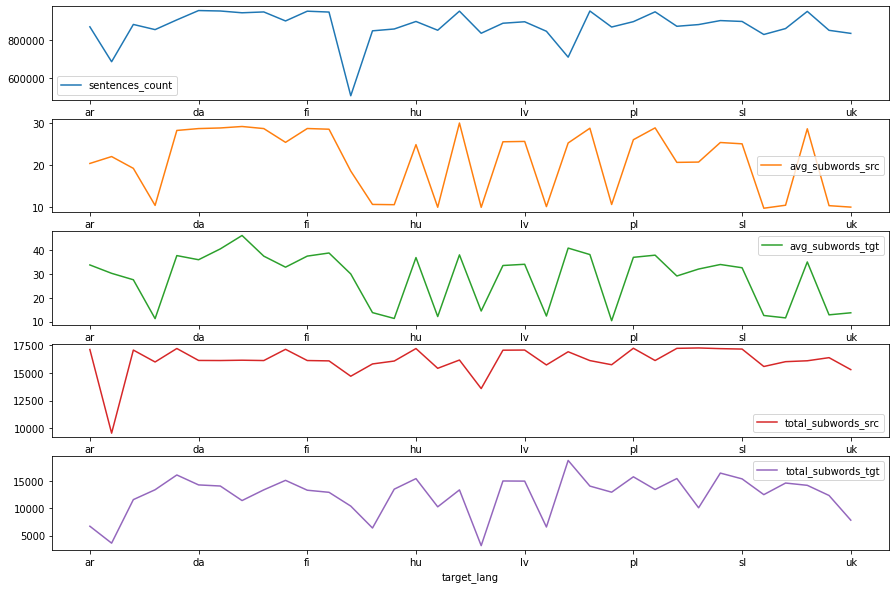
\includegraphics[width=1.0\columnwidth]{img/train_set_statistics.png}
	\mycaption{Training data language statistics}{
		Languages are on the $X$ axis sorted as in \cref{att:list_en-to-36}.
		From top to bottom:
		total number of sentence pairs in training set per language,
		average number of subwords per sentence on the source side,
		the same on the target side,
		total number of unique subwords for this target language on the source side,
		the same on the target side.
	}
	\label{fig:language_statistics}
\end{figure}



\subsection{\todo{UN parallel corpus: English to 5 languages}}
\label{subsection:en-to-5}

\todo{as I show en-to-5 results in RANDOM section, this DS should be here}
\cite{eisele-chen-2010-multiun}


%----------------------------------------------------------------------
\section{Method}
\label{section:method}

In this section we describe how the models are trained, which metrics
are collected and how are they analyzed.


\subsection{\todo{Data preprocessing}}
\label{section:data_preprocessing}

\todo{1. BPE is used, same vocabulary for all models from en-to-36 setup}


\subsection{\todo{Data selection}}
\label{section:data_selection}

\todo{move here resp. parts from training, validation and test}


\subsection{\todo{Training tasks}}
\label{section:training_tasks}

\todo{what is a task, multilingual task, sampling tasks for RANDOM and SIMILAR}


\subsection{\todo{Training}}

For example, let us take \dirmany{En}{Fr, De} setup, which means that
the model to be trained should take a source sentence in English and
produce translation either in French or in German.
The language of model's output depends on the target tag at the beginning
of the input sentence, i.e. \tagto{fr} tag in source sentence leads to French
target.

To train such a model, only related sentence pairs are subsampled
from the whole training set.
In this case, from the whole training set we select only those sentence
pairs which source side starts with tags \tagto{fr} or \tagto{de}.
Such subsampled dataset is then used to train the model.

During the training procedure, once per specified number of updates
occurs the checkpointing of the model.
The model weights are saved to the disk and number of measurements are logged.

\begin{samepage}
\begin{itemize}
	\item [Those measurements are:]
	\item training loss value (mean value for all updates since
	last checkpoint)
	\item learning rate value
	\item training speed (processed words per second)
	\item training time since last checkpoint
	\item number of updates happened from the beginning till this checkpoint
\end{itemize}
\end{samepage}
\begin{samepage}
Hardware usage should also be recorded if possible:
\begin{itemize}
	\item GPU usage
	\item CPU usage
	\item memory usage
	\item disk I/O
	\item network I/O
\end{itemize}
\end{samepage}

The hardware metrics are not important for model's evaluation
but may help early spot mistakes like underuse of GPU or CPU, lack of RAM, etc.
This is why they could possibly be recorded continuously. \todo{link to this point from wandb section}

\subsection{\edit{Validation}}
\label{subsection:validation}

The validation set is used to track model's performance during the training
on an unseen set of data and to perform early stopping.
These measurements are only used during the training and not for the evaluation.

Once per specified number of steps the validation occurs:
validation metrics are recorded, for any metric which value was
improved current model weights are saved as best model by this metric.
If early stopping condition occurred then the training process is stopped.

For any model the validation set is constructed from the big validation set
by selecting only relevant sentence pairs in the same way as the training set,
i.e. pairs with the target in one of the examined languages.
For the example setup from above, \dirmany{En}{De,Fr}, the validation set
consists of an equal amount of \dir{En}{De} and \dir{En}{Fr} sentence pairs.
E.g. if in the complete validation set there are 1000 sentence pairs for
each of possible target languages, then for \dirmany{En}{De,Fr}
model the validation set will contain 2000 sentence pairs, and for
\dirmany{En}{De,Es,Fr} it will contain 3000 sentence pairs.

For the validation set, we collect not only the loss function value
but also the metric of interest, which is \acrshort{bleu} score.
However, this \acrshort{bleu} scores are not used for the model's
evaluation but only during the training process.
The \acrshort{bleu} of the whole model's validation set
is not something we are interested in.
For the discussed example we collect validation bleu:fr and bleu:de scores
which represent \acrshort{bleu} scores for French and German
parts of validation set.
E.g., to compute bleu:fr we select only En\to{}Fr sentence pairs from the
validation set.

Also, an aggregated value of the bleu:xx scores, i.e. the mean of BLEU scores
over all target languages of the current model, is also recorded
and may be used for early stopping: ending the training process
when the metric is not improved during last N validation steps.

\begin{samepage}
Altogether, the following validation metrics are recorded after the
validation step:
\begin{itemize}
	\item loss function value
	\item bleu:xx which is \acrshort{bleu} score for each of
	model's target languages
	\item aggregated value of all bleu:xx values
	\item translation time of the model's validation set
\end{itemize}
\end{samepage}

\subsection{\todo{Finishing the training}}
\label{section:finishing-the-training}

When should we stop the training?
It is not possible to say precisely when did the model
acquire its best performance because of stochastic nature of
the training algorightm (\acrshort{sgd}).
Because of that we need to use some method to decide when
training process should be stopped.


\subsubsection*{Number of \glspl{epoch}}

\todo{First occurence of a term to be italic}
The easiest approach is to specify the number of \glspl{epoch}
after which the training is stopped.
This could be a good solution for the case when all models
that will be compared are trained on the same amount of data from
the same domain.
But in our case, adding one more target language adds a constant
amount of sentence pairs to the training set.
Roughly, if the number of \glspl{epoch} is specified as a stop
condition, a bilingual \dir{En}{De} model will see the German
training data $x$ times, when multilingual \dir{En}{De, Fr, Es}
will only see the German training data $x / 3$ times.

%What value should be used to compare model's performace in time?
%The first and the most obvious approach 
\subsubsection*{Early stopping}

\Gls{early-stopping} is a regularization technique used to avoid
possible \gls{overfitting} of a model on the training data.
In general, it works in the following way: after every validation step
it checks if the metric value improved during last $N$ validations.
The metric to be controlled and number of validation steps $N$ are
the parameters of this method
(see \cref{fig:early_stopping}).

Another situation is even more probable in the area of NMT with generally
large training datasets: model's validation performance
is either stalled or slightly improved
(see \cref{fig:early_stopping_no_improvement}).
In this case \gls{early-stopping} helps to avoid unnecessary spendings
on computational resources.

\begin{samepage}
\begin{figure}[h]
	\centering
	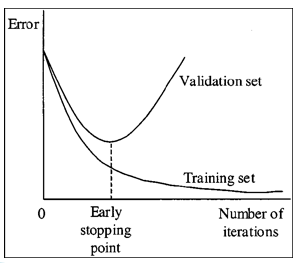
\includegraphics[width=0.6\columnwidth]{img/early_stopping.png}
	\mycaption{\Gls{early-stopping} to prevent overfitting}{
		At the `early stopping' point the model's performance
		on unseen validation set of data does not improve
		anymore. Further training leads to poorer performance
		on unseen data. Stopping the training at this point
		results in better model's performance on unseen data.
	}
	\label{fig:early_stopping}
\end{figure}

\begin{figure}[h]
	\centering
	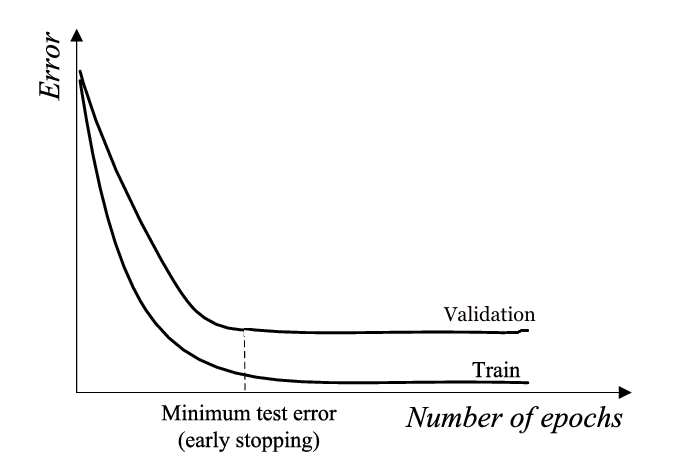
\includegraphics[width=0.6\columnwidth]{img/early_stopping_no_improvement.png}
	\mycaption{\Gls{early-stopping} as the model is not improving}{
		Even though the metric value on the training set is
		still slowly improving, the its value on the unseen
		validation set is stalled. Further spending of 
		computational resources is unjustified.
	}
	\label{fig:early_stopping_no_improvement}
\end{figure}
\end{samepage}

In our case we could use \gls{early-stopping} to ensure more equal conditions
for models with different sizes of training data.
A suitable number $N$ could be found experimentaly, but which metric should be used?

\todo{cross-entropy, perplexity; they may not represent the model's
performance, what about BLEU}

Given that the task is to train a model that is as good as possible in
\textbf{every} of its target directions, the \acrshort{bleu} score of
the whole translated validation set for this set of languages does not
say anything about the model's performance in each specified
translation direction.

\subsubsection*{Aggregated value of BLEU scores}

Therefore, we should use separate BLEU scores which represent
model's performance in each of translation directions.
The most intuitive and naive way is to compare BLEU scores
for each target language.

However, most of frameworks and toolkits can monitor only one metric
for the early stopping.
Considering that different validation \acrshort{bleu} scores
are computed for different parts of the validation set and in
which are in different languages, they cannot be directly compared
and may have different scale.

For example, a model for the \dirmany{En}{De,Fr} direction is being
trained.
Before the moment, an \dir{En}{De} model has already been trained and
had the best \acrshort{bleu} score of 25 on the German part of the
validation set.
A \dir{En}{Fr} model has also been trained, and its result on the
French part of the validation score is 35.
So for the currently training \dirmany{En}{De,Fr}, one percentage point
change for the \dir{En}{De} direction is not equal to the same change for the
\dir{En}{Fr} direction.

Geometric mean is known to be good for aggregating multiple metrics
with different scale (see \cref{eq:geometric_mean}).

\XXX{initially I wanted to achieve what was in the removed paragraph,
but it did not happen (in some cases one of BLEU scores goes a bit down),
so I have replaced it with this version}

\begin{equation}
\label{eq:geometric_mean}
	geometric\_mean = \left(\prod _{i=1}^{n}x_{i}\right)^{\frac {1}{n}}={\sqrt[{n}]{x_{1}x_{2}\cdots x_{n}}}
\end{equation}

\subsection{\edit{Testing}}
\label{subsection:testing}

After the training is finished, the received models should be evaluated on unseen
test data.
For experiments with \gls{en-to-5} dataset (Section \ref{subsection:en-to-5})
the test sets are created in the same way as validation sets.
For \gls{en-to-36} dataset (Section \ref{subsection:en-to-36})
the test set is divided on subsets by the source dataset.
It means, that each of source datasets (like OpenSubtitles/v11, 
Europarl/v7, etc.) there exists a separate test set.
So after translating the test set for each of target directions of the model
the following record is created:
\begin{itemize}
	\item model name
	\item source language
	\item target languages
	\item tested target language
	\item \acrshort{bleu} score for this part of translation
	\item metric, based on which the best model was saved
	\item dataset name (for \gls{en-to-36})
\end{itemize}

Let us return to the example setup is En\to{}$\{$De, Fr$\}$ and
suppose the reported validation metrics are the mean loss function value on
test set and 'translation' (geometric mean of all reported BLEU scores,
see Section \ref{subsection:validation}).
After the training is finished, there will be two models: best by
loss value and best by 'translation'.
For each of those two records are created: for En\to{}Fr translation
and for En\to{}Es. In total, 4 results are recorded.

If the model was trained and tested on \gls{en-to-36} dataset,
than 4 times \textit{n} records are created, where \textit{n}
is number of OPUS subdatasets from which the data was sampled.


\subsection{Analysis}

After required set of models is trained and their test
metrics are collected, data should be analysed.

For example, let us take these four models: \dirmany{En}{De, Fr},
\dirmany{En}{De, Az}, \dirmany{En}{De, Bg}, and \dirmany{En}{Bg, Az}.
After the training, they provide us with three results for \dir{En}{De}
direction 2-target baseline,
one value for \dir{En}{Fr},
two values for \dir{En}{Bg}
and two for \dir{En}{Az}.
These aggregated \dirmany{En}{De, X} results will be later compared with
aggregated \dirmany{En}{De, X1, X2} for three target languages,
\dirmany{En}{De, X1, X2, X3} for four target languages, where X1, ... X$i$ are
some other targets.

Next, the \dirmany{En}{De, RANDOM} notation refers to a multilingual
model that was trained in the RANDOM experiment (randomly selected targets),
where one of the targets is German.
In the same way, \dirmany{En}{De, GERMANIC} refers to a model from
the GERMANIC experiment (targets selected from Germanic languages list).


%----------------------------------------------------------------------
\section{Training tools}

In the following section we describe the tools that are uset to implement
what was shown in Section \ref{section:method}.

\subsection{Toolkits}

There exists a number of different tools that can be used for training a NMT model.
General purpouse deep learning programming libraries like
Tensorflow\footnote{\url{https://tensorflow.org/}} and
PyTorch\footnote{\url{https://pytorch.org/}} are most popular for deep learning related
research. With their help it is possible to construct any of today's state-of-the-art
NMT models; pre-built and pre-trained models are initially present in such frameworks,
but it is also possible to describe a model from scratch.

Another option is presented by specialized NMT tool kits.
They usually contain efficient and tested implementations of NMT models as well as some of
usefull preprocessing tools.
For the experiments described in \ref{section:experiments} there is a need to train significant
amount of models with the same architecture and settings but different datasets.
Due to that fact, in this work the use of specialized NMT tool kit is more suitable.
Let us consider the foolowing list of broadly used tool kits as for year 2020,
presented in \cite{koehn_2020}:

\begin{itemize}
  \item OpenNMT (based on Torch/pyTorch)\footnote{\url{https://opennmt.net}}
  \item Sockeye (based on MXNet)\footnote{\url{https://github.com/awslabs/sockeye}}
  \item Fairseq (based on pyTorch)\footnote{\url{https://github.com/pytorch/fairseq}}
  \item Marian (stand-alone implementation in C++)\footnote{\url{marian-nmt.github.io}}
  \item Google's Transformer (based on Tensorflow)\footnote{\url{
    https://github.com/tensorflow/models/tree/master/official/transformer}}
  \item Tensor2Tensor (based on Tensorflow) \footnote{\url{
    https://github.com/tensorflow/tensor2tensor}}
\end{itemize}

We chose \textit{MARIAN-NMT} tool kit\footnote{\cite{mariannmt}} as a fast solution
with stable and efficient \textit{Transformer} \cite{vaswani-2017-transformer} implementation,
minimum of third-party dependencies, and ability to train models on multiple GPU units in parallel.


\subsection{Computational cluster}

In the experiments proposed above the expected number of models to be trained is quite big.
First of all, there should be 36 models for \textit{mono-target baseline} for En\to{}36 dataset.
For \textit{multi-target random} experiment the number is much bigger.
For example, let us consider a case with En\to{}3 models - each model translates from English to 
3 target languages. Specifying that each of 36 target languages from En\to{}36 dataset
should appear at least in 3 En\to{}3 models, series of random generation of En\to{}3 setups gave
the smallest amount of such setups equal to 44. For En\to{}5 case with 5 target languages in each
model and with the same restriction of minimum occurance the same procedure gave the
minimum amount of needed models equal to 34.

To be able to train large number of models in a reasonable amount of time we needed to use
computational cluster with GPU cards.
The computational clusters available at the institution are operating under
SGE\footnote{\url{https://arc.liv.ac.uk/trac/SGE}} scheduling software and are equipped with
GPU cards with minimum CUDA \textit{compute capability} 6.1.

Considering data storage quota limitation and high utilization of computational resources by
the cluster's users, the following training pipeline was designed:

\begin{outline}
    \1 Prepare task list
    \1 Iterate over the list working with at most N tasks in parallel
    \1 For each task
        \2 Subsample the dataset taking only those sentence pairs with target languages
	   specified in the task
	\2 Run the training procedure for limited amount of time (e.g. for one hour only)
	   starting with previous checkpoint if it already exists
	\2 Regularly compute metrics on the developement set and report them
	\2 On the event of evaluation on the developenemt set save the best model for each metric
	\2 After time is out the training is stopped and subsampled datasets are removed
    \1 If for next selected task the model is already trained then select next task from the list
    \1 If for next selected task the model is currently being trained then decrease
       the number N of tasks processed in parallel
\end{outline}


\subsection{Inspecting the training process}

As the number of models trained and being trained is growing, monitoring of the training
process becomes more and more complicated. If the experiments are also being run on different
computational clusters it becomes very possible that a parameter mistakenly set up to different
value or a corrupted dataset, or even hardware version may lead to an unexpected difference in results.

To address these and other issues that may occur during the training process we use
Weights$\&$Biases\footnote{\cite{wandb}} experiment tracking tool.
Its main features that are useful in this prospective are following:
\begin{outline}
	\1 Metric visualization
		\2 Training and validation loss curves
		(Figure \ref{fig:single-lang-group-vs-random-dashboard} left subplot)
		\2 Scatter plots (Figures \ref{fig:inspect-convergence}
		and \ref{fig:single-lang-group-vs-random-dashboard} middle subplot)
	\1 Artifact storage
		\2 Model checkpoints storage
			\3 stores 'heavy' model files which cannot be stored
			in \emph{git}
			\3 along with \emph{git} it makes possible to move training
			to the different computational cluster system
		\2 Sample translations of validation set
			\3 helps to observe improvements of translation quality
			in time
			\3 lets verify that model is actually produces meaningfull
			translation
	\1 Customizable reports
	\1 Hardware utilization
\end{outline}

\begin{sidewaysfigure}[b]
	\centering
	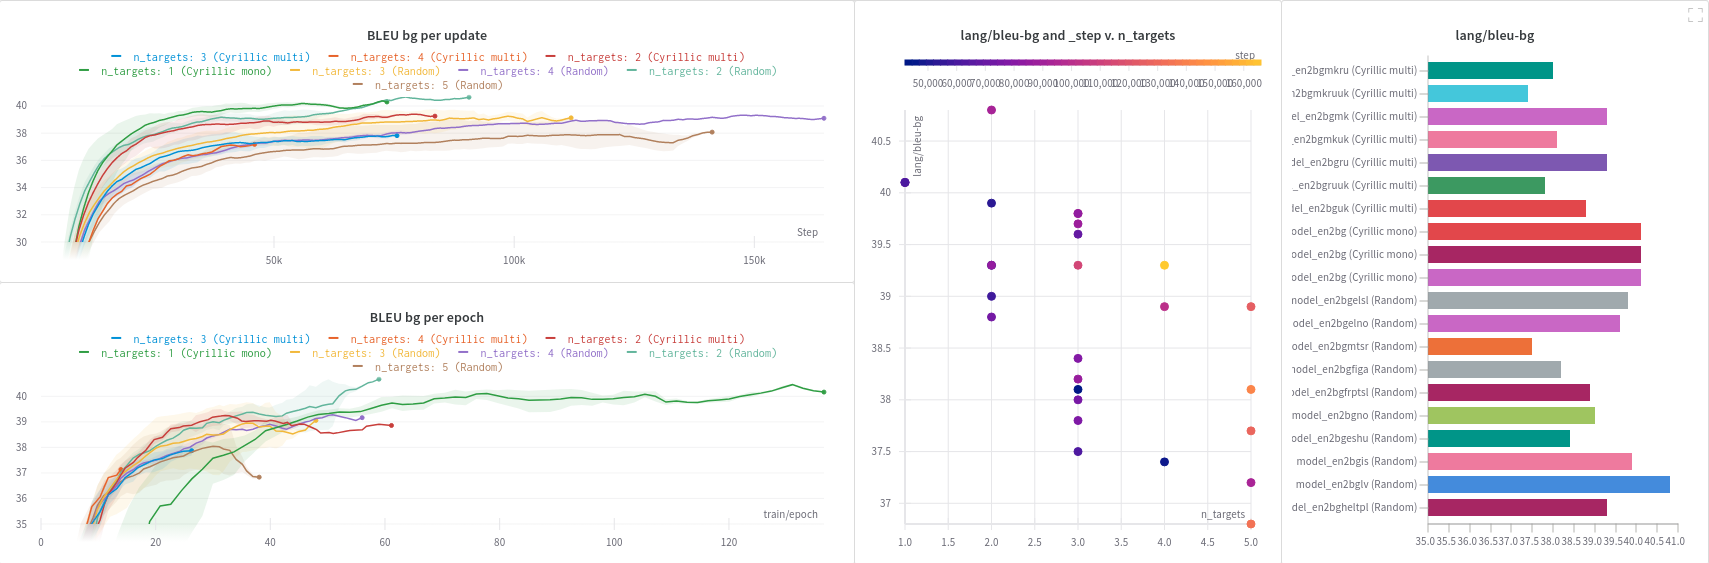
\includegraphics[width=1.0\columnwidth]{img/slavic_cyrillic_bg.png}
	\mycaption{%
		Training progress dashboard for one translation direction%
	}{
		Here is a part of interactive report for `Slavic languages
		with Cyrillic script vs. random' experiment.
		In this specific case models' performance on Bulgarian part of
		validation set is compared. Note: the visualized BLEU scores are only
		used during the training and are not used for evaluation.

		\emph{Left}: \acrshort{bleu} score for \dir{En}{Bg} translation direction is monitored with
		training step on $X$ axis (top) and training epoch  (bottom).
		Each curve represents mean value (line) and its min/max value
		(range) at the point of time of multiple models' results.
		Models are grouped by the number of target languages and experiment subgroup
		(bilingual \dir{En}{Bg}, multilingual \dirmany{En}{Slavic} and \dirmany{En}{Random}).

		\emph{Middle}: Number of targets (axis $X$) vs.
		\acrshort{bleu} on \dir{En}{Bg} validation set (axis $Y$) vs.
		update steps (colos with scale at the top).

		\emph{Right}: Individual models' \dir{En}{Bg} validation \acrshort{bleu} scores.
	}
	\label{fig:single-lang-group-vs-random-dashboard}
\end{sidewaysfigure}


\begin{figure}[h]
	\begin{minipage}{0.8\textwidth}
	\centering
	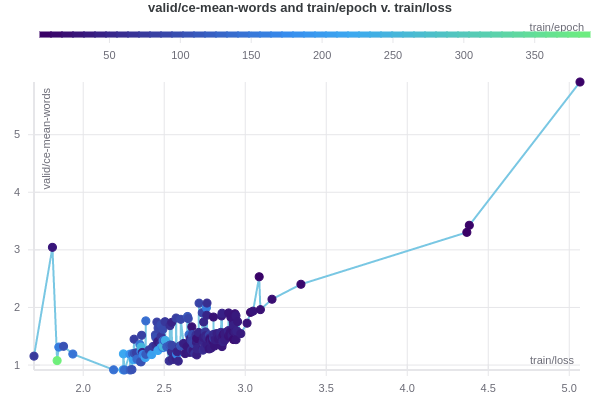
\includegraphics[width=1.0\columnwidth]{img/inspect_overfit.png}
	\end{minipage}\hfill
	\begin{minipage}{0.8\textwidth}
	\centering
	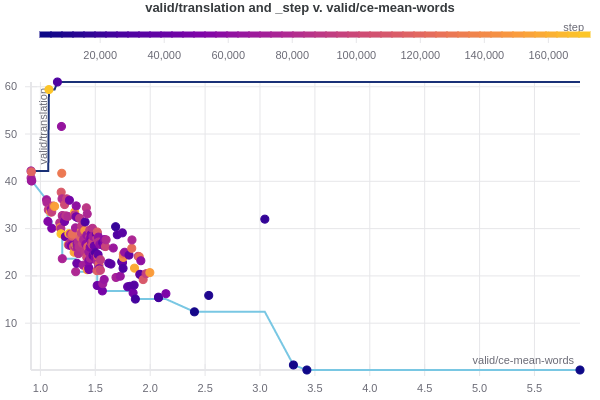
\includegraphics[width=1.0\columnwidth]{img/inspect-bleu-vs-loss.png}
	\end{minipage}
	\mycaption{%
		Overall convergence dashboard%
	}{
		In these two interactive graphs, each point represents one model.
		Models that are currently training are visualized here together with
		completely converged models and those which training process is currently
		on hold.

		\emph{Top}: the $X$ axis represents the training loss value,
		the $Y$ axis represents the value for the same loss function calculated
		on the validation set. The color of each point represents current training
		epoch for the model. Normally for any model the point \fix{moves} from top right
		part of this graph to the bottom left part, representing both training and
		validation loss being gradually decreased during the training procedure.
		The point that moves to the middle left part of the graph may signalize about
		either \gls{overfitting} of the model on training set, or difference in data
		distribution in training and validation set, or else some mistake in training
		settings.
		This is useful for finding which training runs need attention and perhaps debugging.

		\emph{Right}: in this plot loss value on the validation set (axis $X$)
		is compared with geometric mean of \acrshort{bleu} scores
		for each of target languages.
		For any model during the training, its point usually \fix{move} from
		bottom right corner into the cluster of other points.
		The model the point of which `arrives' to any other location than
		the cluster may need special attention.
	}
	\label{fig:inspect-convergence}
\end{figure}


\cleardoublepage

\subsection{\todo{Model settings}}

The initial parameter selection is made with respect to \cite{training-tips}.
First of all, the hyperparameters of MT model are tuned
on couple of language pairs from one dataset.
The parameters leading to the same result in shorter time were preferred.
Then the selected parameters were used on all experimends with the dataset.


\subsubsection*{Tuning early stopping on early runs}

The initial \gls{early-stopping} setting was that after 5 consecutive
validation steps without improvement of validation \gls{loss} value
the training process stopped.
However, during the training of the first couple of bilingual models
the following situation has happened quite often:
further improving performance on validation set by
couple of tenths of BLEU points took as much time as reaching
the pre-optimal state.

In the \cref{fig:no_improvement_de}, it  can be seen that the path from
the beginning of training to the optimal point B (26.9 \acrshort{bleu})
took as much time as its further improvement by 0.2 BLEU
at point D (27.1 \acrshort{bleu}). However, there were certain models
with a bit bigger improvement after a much longer time, e.g.
0.8 \acrshort{bleu} points on Figure \ref{fig:no_improvement_fi}.

This behaviour makes our decision on where to stop particularly
complicated for multilingual models, as discussed in
\cref{section:finishing-the-training}.
After considering also some of preliminary multilingual runs,
the `patience' parameter of \gls{early-stopping} was set to 15.
After 15 consequtive validation steps without a metric improvement,
the training process is stopped.

\fix{it needs to be presented earlier and *commented including motivation*.
The red lines are unnatural at the first sight.}
In order to visually highlight when an increase in the validation score
is observed, we plot the number of ``steps stalled'',
see the red line in \cref{fig:no_improvement_de}.
The higher the diagonal line grows, the longer we have to wait for an improvement.
For instance, we see that the path..from beg to B took...

\begin{figure}[p]
	\centering
	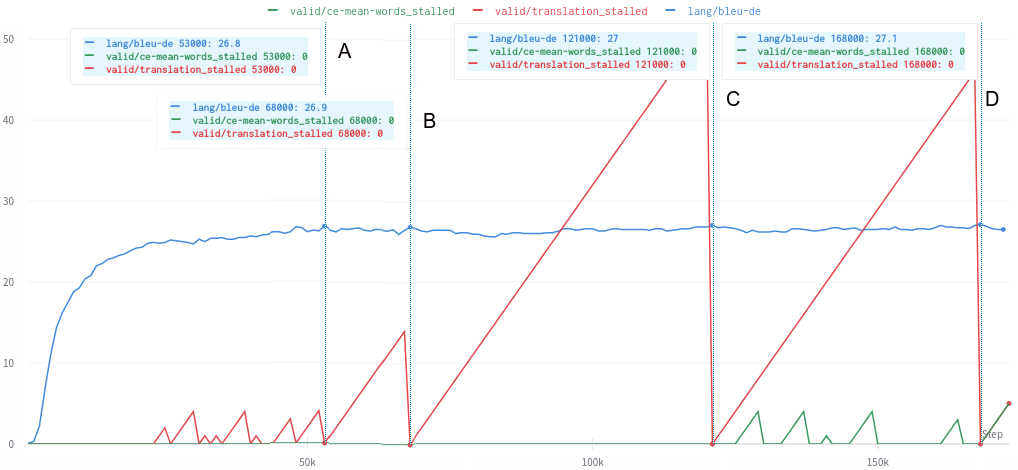
\includegraphics[width=1.0\columnwidth]{img/no_improvement_de.png}
	\mycaption{Example change of model's performance on validation set
		   in time}{
		Preliminary \dir{En}{De} model.

		\textit{Blue}: validation metric (value on the left axis in BLEU)

		\textit{Red}: validation metric (BLEU) stalled.
		Each consecutive validation step when the metric
		is not improved this value is incremented by 1.
		When the metric is improved this value is reset to 0.

		\textit{Green}: loss function value on validation set is
		stalled. Same logic as for \textit{Red}.

		BLEU score values at the points of improvement:
		$A$ -- 26.8, $B$ -- 26.9, $C$ -- 27.0, $D$ -- 27.1.
	}
	\label{fig:no_improvement_de}

	\vspace*{\floatsep}% https://tex.stackexchange.com/q/26521/5764

	\centering
	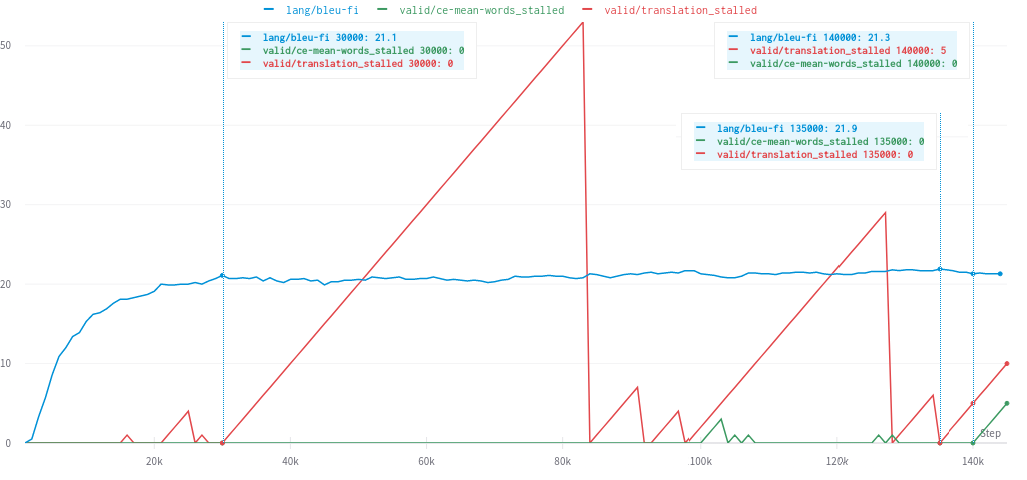
\includegraphics[width=1.0\columnwidth]{img/no_improvement_fi.png}
	\mycaption{Small improvement during long training}{
		In this case (\dir{En}{Fi}), the difference is a bit more
		visible: 21.3 at the first point and 21.9 at the best.
		Colors and scales are the same as at
		Figure \ref{fig:no_improvement_de}.
	}
	\label{fig:no_improvement_fi}
\end{figure}

\chapter{Bilingual and multi-lingual baselines}

In this chapter we describe the baseline experiments.
Bilingual baselines are needed to specify the starting point:
how good model can perform on specific translation direction
for each test set.

After bilingual results are collected and inspected, it is time for
multi-lingual baselines. As multi-lingual baselines we consider models
with randomly selected set of target languages. This way we can see
how much adding more target languages to the model changes its performance
on the same specific translation direction.


\section{\todo{Bilingual baseline}}
\label{section:bilingual_baseline}


\begin{figure}[h]
	\centering
	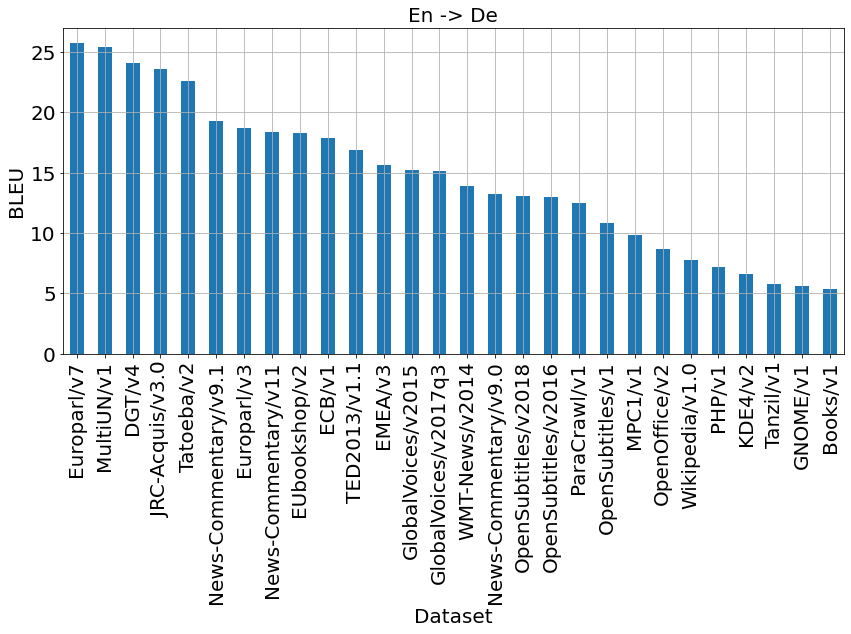
\includegraphics[width=0.9\columnwidth]{../img/bilingual_en_de.png}
	\mycaption{En\to{}De bilingual results}{
		Datasets on the \emph{X} axis are sorted by declining BLEU score.
	}
	\label{fig:bilingual_en_de}
\end{figure}


\section{\todo{Multilingual baseline}}
\label{section:multilingual_baseline}

\begin{figure}[h]
	\centering
	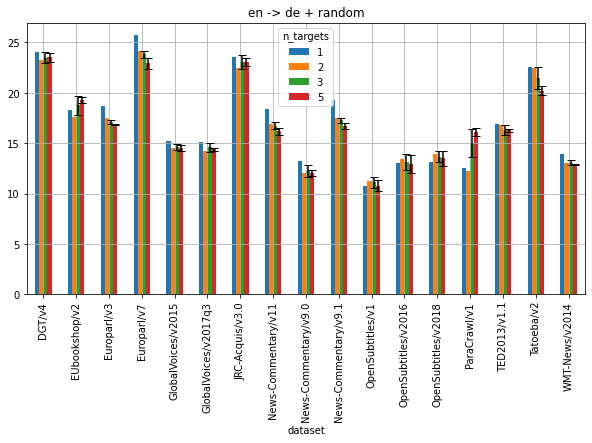
\includegraphics[width=0.9\columnwidth]{../img/random_en_de2.png}
	\mycaption{En\to{}De monolingual baseline results (RANDOM)}{
		Datasets with BLEU lower than 10 are removed
	}
	\label{fig:random_en_de}
\end{figure}

E.g. as a bilingual baseline model for German target language the En\to{}De
model is trained.
En\to{}De,Fr, En\to{}${De,Az}$, En\to{}${De,Bg}$ En\to{}${Bg,Az}$ models
provide us with 3 results for En\to{}De direction 2-target baseline, as well
as one value for En\to{}Fr, two values for En\to{}Bg and two for En\to{}Az.
These aggregated En\to{}${De,X}$ results will be later compared with
aggregated En\to{}${De,X1,X2}$ for 3 target languages,
En\to{}${De,X1,X2,X3}$ for 4 target languages, where X1, ... X\textit{i} are
randomly selected languages.
Also in the next chapters these results will serve as a baseline for
aggregated En\to{}${De,Y1,Y2...}$ results of N target languages for languages
Y\textit{i} being from some group of languages similar to De.

\section{Expected results}

As we have seen in section \ref{section:multitarget_theory}, models with more languages
in the mix usually perform slightly or significantly worse than bilingual ones.
Also, for bilingual baselines no significant change in performace is expected with adding
the target language tags.

However, there might be different unexpected effects due to slight domain-wise differences
in corpora content for different target languages.

\section{Performance drop on massively multilingual setup}
1-to-3, 5, 7, etc. models on en-to-36 dataset (0.9 mil. sentences per target language)

When the size of the model is fixed, adding more translation directions usually causes
worsening of its performance. Multiple studies have shown this to be truth for
many-to-many setup.



\begin{table}[h!]
\begin{subtable}[t]{0.45\linewidth}
	\centering
	\begin{tabular}{rrrr}
	\toprule
	n\_targets &   mean &   std & count \\
	\midrule
	         1 &  41.40 &  ---  &   1 \\
	         2 &  40.60 &  0.20 &   3 \\
	         3 &  39.39 &  0.62 &   8 \\
	         4 &  39.40 &  0.71 &   2 \\
	         5 &  38.45 &  0.52 &   6 \\
	\bottomrule
	\end{tabular}

	\caption{
		En\to{}Bg for \emph{Europarl/v7} dataset.
		}
	\label{tab:bg/Europarl/v7}
\end{subtable}
\begin{subtable}[t]{0.45\linewidth}
	\centering
	\begin{tabular}{rrrrrrr}
	\toprule
	n\_targets & mean & count & std \\
	\midrule
	        1 &     19.50 &    1 &   --  \\
	        2 &     18.88 &    4 &  0.39 \\
	        3 &     17.45 &    4 &  0.52 \\
	        4 &     17.80 &    2 &  0.42 \\
	\bottomrule
	\end{tabular}
	
	\caption{
		En\to{}Ru for \emph{OpenSubtitles/v2016} dataset.
		}
	\label{ table:ru/OpenSubtitles/v2016 }
\end{subtable}
\mycaption{\acrshort{bleu} score change with adding target languages}{
    (a) First row: for mono-lingual En\to{}Bg model test \acrshort{bleu} score is 41.40.
    Second row: for 3 (column \emph{count}) En\to{}Any
    models with two target languages
    (column \emph{n\_targets}) one of which is Bulgarian
    the mean \acrshort{bleu} score is 40.60 with standard deviation 0.20.
    (b): same way as (a)
}
\end{table}



% \begin{table}[h]
% \centering
% \begin{tabular}{rrrrrrr}
% \toprule
% n\_targets & mean & count & std \\
% \midrule
%         1 &     --.-- &    1 &    -  \\
%         2 &     18.86 &    8 &  0.31 \\
%         3 &     17.59 &    8 &  0.48 \\
%         4 &     17.80 &    4 &  0.35 \\
% \bottomrule
% \end{tabular}
% 
% \caption{
% 	\acrshort{bleu} score for En\to{}Ru translation on test set part of
% 	\emph{OpenSubtitles/v2016} dataset.
% 	Description is the same as for table \ref{tab:bg/Europarl/v7}
% 	}
% \label{ table:ru/OpenSubtitles/v2016 }
% \end{table}

\section{Performance decrease on richer data sets}
1 to 3, 4, 5 on UN corpus (much more sentence pairs per target language)
\cite{eisele-chen-2010-multiun}

\begin{table}[h!]
\centering
\begin{tabular}{r|c}
\toprule
model         & BLEU  \\
\midrule
m.esfrru t.ru & 40.35 \\
m.esru t.ru   & 42.16 \\
m.frru t.ru   & 41.95 \\
m.ru t.ru     & 44.20 \\
m.esfrru t.fr & 45.03 \\
m.esfr t.fr   & 46.84 \\
m.frru t.fr   & 45.66 \\
m.fr t.fr     & 48.64 \\
m.esfrru t.es & 56.33 \\
m.esfr t.es   & 57.94 \\
m.esru t.es   & 57.31 \\
m.es t.es     & 59.94 \\
\bottomrule
\end{tabular}
\end{table}

\chapter{Group by language groups}
\label{section:experiment_groups}


In this section we describe the results of the multilingual models with related target languages, i.e.: 1 to 2, 3, 4, 5, etc. models on en-to-36 dataset (0.9 mil. sentences per target language)
compared with random runs.


%----------------------------------------------------------------------
\section{Germanic group}
\label{section:germanic_group}

Here Germanic group consists of German, Dutch, Swedish, Danish, Norwegian and Islandic.
Models \dirmany{En}{Germanic} are compared to \dirmany{En}{non-Germanic}, where non-Germanic consists
of any langauge except of the languages from the Germanic group.
In \cref{fig:de_random_vs_germanic} and \cref{fig:da_random_vs_germanic}, some selected
results are visualized along with vocabulary changes. Results for OpenSubtitles/v2018 mean
the \acrshort{bleu} score on test set part was sampled from OpenSubtitles/v2018.
In both figures, the subfigure (a) shows the result for spontaneous or pseudo-spontaneous speech
transcripts, i.e. subtitles, while sub-figure (b) shows the result for prepared
speeches or documents from Europarl or UN meetings.

In this cases observations are twofold:
\begin{itemize}
	\item For test sets with lower bilingual \acrshort{bleu} score,
		adding more target languages to the model improves the score;
		adding related target languages improves it even more.
	\item Adding more target languages improves translation result on test
		sets from spontaneous speech domain
		but worsens them for prepared speech or documents.
\end{itemize}

From the (c), we can see, that when comparing the vocabulary size of models
where languages related to the
target German are added with models where random languages are added,
the vocabulary clearly grows faster with random languages.
This behaviour is expected and confirms that related languages contain
similar patterns of subwords.

\begin{figure}[h]
	\subcaptionbox{OpenSubtitles/v2018, the baseline is
			the bilingual score: 13.1 \acrshort{bleu}}[0.48\textwidth]{
		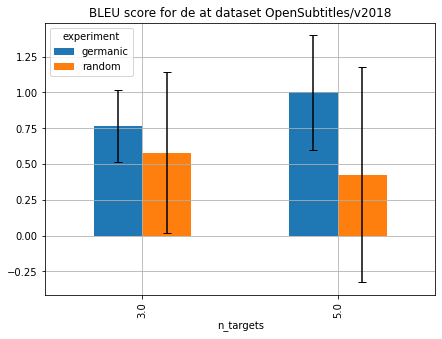
\includegraphics[width=0.48\textwidth]{img/de_opensubtitles_13_1.png}
	}\hfill
	%\vspace*{\floatsep}% https://tex.stackexchange.com/q/26521/5764
	\subcaptionbox{MultiUn, bilingual score: 25.4 \acrshort{bleu}}[0.48\textwidth]{
		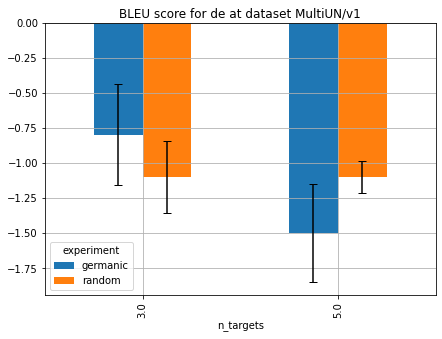
\includegraphics[width=0.48\textwidth]{img/de_multiun_25_4.png}
	}

	\begin{minipage}{0.48\textwidth}
		\mycaption{En\to{}De \acrshort{bleu} score difference: Random vs. Germanic}{
			On $X$ axis is the number of target languages.
			On $Y$ axis id the difference score when comparing with bilingual baseline
			\acrshort{bleu}.
			Black vertical lines show standard deviation across the
			runs we sampled.
			(a) Adding random target languages as well as related ones slightly
			improves German translation score on speech transcript.
			(b) Adding neither random target languages nor related ones helps with
			prepared speeches transcripts and documents in German.
			(c) Adding a related target language into the mix introduces
			fewer new unique subwords.
		}
		\label{fig:de_random_vs_germanic}
	\end{minipage}\hfill
	\subcaptionbox{Subword dictionary size used for target side}[0.48\textwidth]{
		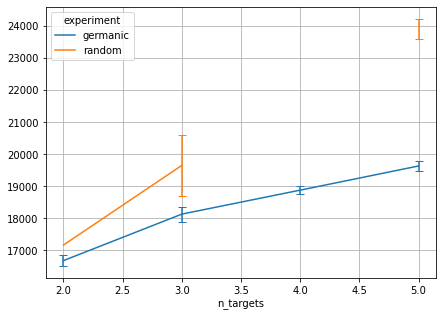
\includegraphics[width=0.48\textwidth]{img/de_tgt_subwords.png}
	}\hfill
	\vspace*{\floatsep}% https://tex.stackexchange.com/q/26521/5764

\end{figure}

\begin{figure}[h]

	\centering
	\subcaptionbox{OpenSubtitles/v2018, bilingual score: 15.6 \acrshort{bleu}}[0.48\textwidth]{
		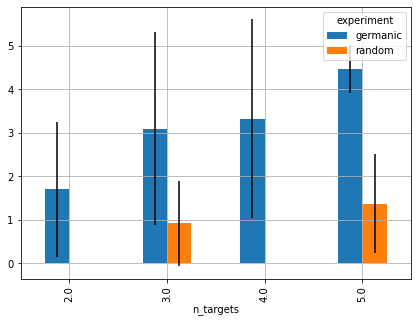
\includegraphics[width=0.48\textwidth]{img/da_opensubtitles_15_6.png}
	}\hfill
	\subcaptionbox{Europarl/v3, bilingual score: 32.5 \acrshort{bleu}}[0.48\textwidth]{
		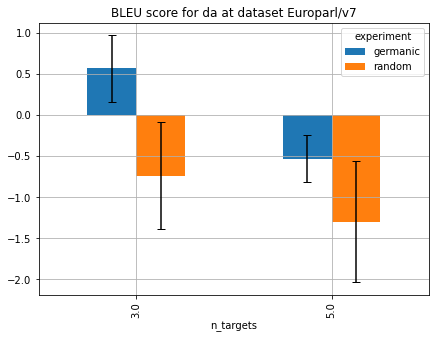
\includegraphics[width=0.48\textwidth]{img/da_europarl_v7_32_5.png}
	}\hfill
	%\vspace*{\floatsep}% https://tex.stackexchange.com/q/26521/5764
	\subcaptionbox{Subword dictionary size used for target side}[0.48\textwidth]{
		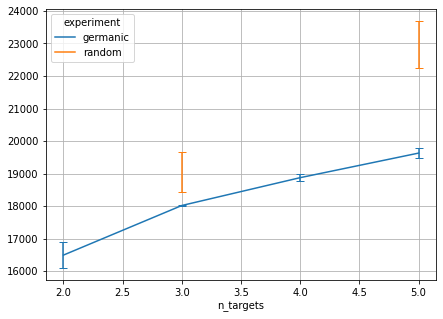
\includegraphics[width=0.48\textwidth]{img/da_tgt_subwords.png}
	}\hfill
	\begin{minipage}{0.48\textwidth}
		\mycaption{\dir{En}{Da} \acrshort{bleu} score difference: Random vs. Germanic}{
		The axis are same as above.
		(a) For OpenSubtitles test set, which consists of human speech transcripts,
		adding similar target language to the mix significantly imporves the result.
		(b) For Europarl/v7 which consists of prepared speeches transcripts and documents,
		adding more Germanic languages to the mix did not worsen Danish translation
		quality (unlike the case with German).
		(c) Adding random target language to the mix adds more subwords to the target
		subword dictionary.
	}
	\label{fig:da_random_vs_germanic}
	\end{minipage}
\end{figure}


\cleardoublepage

%----------------------------------------------------------------------
\section{Slavic with Cyrillic script}
\label{section:cyrillic_group}

The \textit{Slavic with Cyrillic script} group consists of
Bulgarian, Macedonian, Russian and Ukrainian.
Models \dirmany{En}{Cyrillic} are compared to \dirmany{En}{non-Cyrillic},
where non-Cyrillic consists of any language except of those selected from the group above.
In Figures \ref{fig:bg_random_vs_cyrillic} and \ref{fig:ru_random_vs_cyrillic},
some selected results are visualized along with vocabulary changes.
Test sets for subfigures (a) and (b) were
selected the same way as in \cref{section:germanic_group}.

From the two opposite observations of \ref{section:germanic_group} in this case
the second one is observed: low results of bilingual baselines
are getting slightly better or remain the same,
good results are getting slightly or significantly worse as more languages are
added to the mix.

\begin{figure}[h]

	\centering
	\subcaptionbox{OpenSubtitles/v2018, bilingual score: 23.7 \acrshort{bleu}}[0.48\textwidth]{
		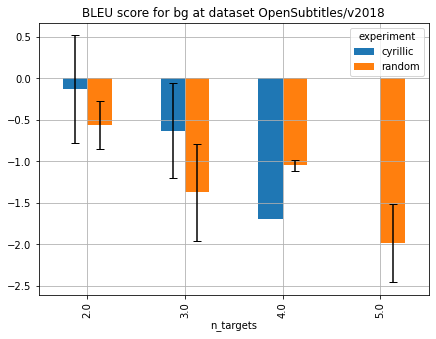
\includegraphics[width=0.48\textwidth]{img/bg_opensubtitles_23_7.png}
	}\hfill
	\subcaptionbox{Europarl/v7, bilingual score: 41.4 \acrshort{bleu}}[0.48\textwidth]{
		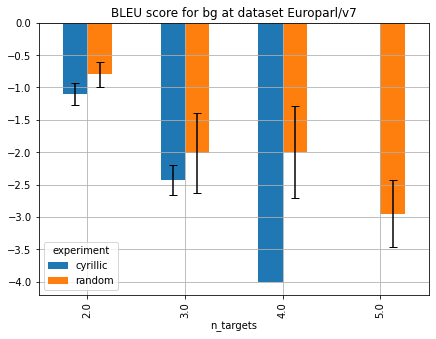
\includegraphics[width=0.48\textwidth]{img/bg_europarl_41_4.png}
	}\hfill
	%\vspace*{\floatsep}% https://tex.stackexchange.com/q/26521/5764
	\subcaptionbox{Subword dictionary size used for target side}[0.48\textwidth]{
		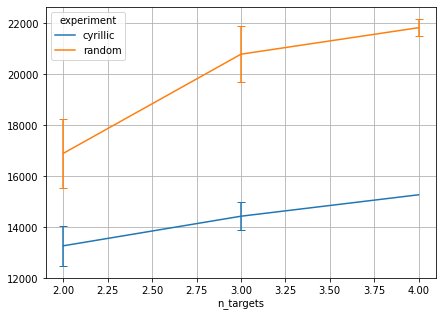
\includegraphics[width=0.48\textwidth]{img/bg_tgt_subwords.png}
	}\hfill
	\begin{minipage}{0.48\textwidth}
	\mycaption{En\to{}Bg \acrshort{bleu} score difference: Random vs. Slavic with Cyrillic script}{
		The axes are same as for Figures \ref{fig:da_random_vs_germanic}
		and \ref{fig:de_random_vs_germanic}.
		There is no data for Cyrillic and 5 targets as there are only
		4 such languages in the en-to-36 dataset.
		Both (a) and (b) show a significant decrease in translation quality
		as more languages are added to the setup.
		In (c) it is clearly visible how adding a random language with
		non-cyrillic script increases target subword vocabulary size.
	}
	\label{fig:bg_random_vs_cyrillic}
	\end{minipage}
\end{figure}

\begin{figure}[h]

	\centering
	\subcaptionbox{OpenSubtitles/v2018, bilingual score: 19.2 \acrshort{bleu}}[0.48\textwidth]{
		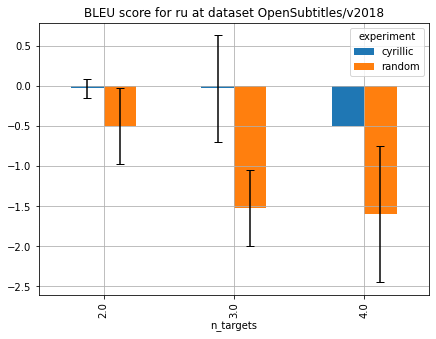
\includegraphics[width=0.48\textwidth]{img/ru_opensubtitles_19_2.png}
	}\hfill
	\subcaptionbox{MultiUN, bilingual score: 14.6 \acrshort{bleu}}[0.48\textwidth]{
		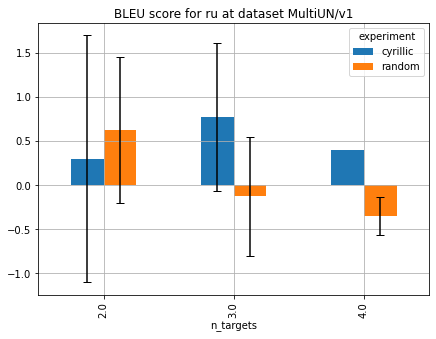
\includegraphics[width=0.48\textwidth]{img/ru_multiun_14_6.png}
	}\hfill
	%\vspace*{\floatsep}% https://tex.stackexchange.com/q/26521/5764
	\subcaptionbox{Subword dictionary size used for target side}[0.48\textwidth]{
		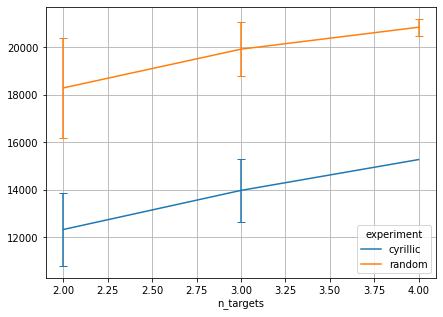
\includegraphics[width=0.48\textwidth]{img/ru_tgt_subwords.png}
	}\hfill
	\begin{minipage}{0.48\textwidth}
	\mycaption{En\to{}Ru \acrshort{bleu} score difference: Random vs. Slavic with Cyrillic script}{
		The axes are same as for Figures \ref{fig:da_random_vs_germanic},
		\ref{fig:de_random_vs_germanic} and \ref{fig:bg_random_vs_cyrillic}.
		There is only one value for Cyrillic with four targets as
		there are only four languages in the selected group.
		Both (a) and (b) show a significant decrease in translation quality.
		In (c), it is clearly visible how adding a random language with
		non-Cyrillic script increases target subword vocabulary size.
	}
	\label{fig:ru_random_vs_cyrillic}
	\end{minipage}
\end{figure}

%\begin{table}[h]
%\begin{subtable}[t]{1\linewidth}
%\begin{tabular}{rrrrrrr}
%\toprule
%n\_targets & \multicolumn{2}{l}{mean} & \multicolumn{2}{l}{count} & \multicolumn{2}{l}{std} \\
%          & cyrillic & random & cyrillic & random &  cyrillic & random \\
%\midrule
%        2 &     14.9 &   15.3 &      6   &    8   &       1.2 &    0.7 \\
%        3 &     15.4 &   14.6 &      6   &    8   &       0.7 &    0.6 \\
%        4 &     15.2 &   14.3 &      2   &    4   &       0.3 &    0.2 \\
%\bottomrule
%\end{tabular}
%\caption{MultiUN/v1}
%\label{table:ru/multi_un}
%\end{subtable}
%\begin{subtable}[t]{1\linewidth}
%\begin{tabular}{rrrrrrr}
%\toprule
%n\_targets & \multicolumn{2}{l}{mean} & \multicolumn{2}{l}{count} & \multicolumn{2}{l}{std} \\
%          & cyrillic &  random & cyrillic & random &  cyrillic &    random \\
%\midrule
%        2 &  22.9    &  22.9   &      6   &    8   &       0.5 &       0.5 \\
%        3 &  22.3    &  21.0   &      6   &    8   &       0.3 &       0.7 \\
%        4 &  21.1    &  20.9   &      2   &    4   &       0.5 &       0.5 \\
%\bottomrule
%\end{tabular}
%\caption{NewsCommentary/v11}
%\label{table:ru/news_v11}
%\end{subtable}
%\begin{subtable}[t]{1\linewidth}
%\begin{tabular}{rrrrrrr}
%\toprule
%n\_targets & \multicolumn{2}{l}{mean} & \multicolumn{2}{l}{count} & \multicolumn{2}{l}{std} \\
%          &   cyrillic &   random & cyrillic & random &  cyrillic &    random \\
%\midrule
%        2 &  19.266667 &  18.7375 &      6.0 &    8.0 &  0.273252 &  0.396187 \\
%        3 &  19.350000 &  17.7875 &      6.0 &    8.0 &  0.653452 &  0.418970 \\
%        4 &  18.900000 &  17.5750 &      2.0 &    4.0 &  0.282843 &  0.613052 \\
%\bottomrule
%\end{tabular}
%\caption{OpenSubtitles/v2018}
%\label{table:ru/news_v11}
%\end{subtable}
%\caption{Mean \acrshort{bleu} score, its standard deviation and number of trained models (count) for Russian at various datasets}
%\end{table}
%
%
%
%\begin{table}[h]
%\begin{subtable}[t]{1\linewidth}
%\begin{tabular}{rrrrrrr}
%\toprule
%n\_targets & \multicolumn{2}{l}{mean} & \multicolumn{2}{l}{len} & \multicolumn{2}{l}{std} \\
%          &   cyrillic &     random & cyrillic & random &  cyrillic &    random \\
%\midrule
%        2 &  40.433333 &  40.683333 &      6.0 &    6.0 &  0.273252 &  0.183485 \\
%        3 &  39.216667 &  39.506250 &      6.0 &   16.0 &  0.318852 &  0.611521 \\
%        4 &  37.750000 &  39.450000 &      2.0 &    4.0 &  0.494975 &  0.525991 \\
%        5 &        NaN &  38.483333 &      NaN &   12.0 &       NaN &  0.511386 \\
%\bottomrule
%\end{tabular}
%\caption{Europarl/v7}
%\label{ table:bg/Europarl/v7 }
%\end{subtable}
%\begin{subtable}[t]{1\linewidth}
%\begin{tabular}{rrrrrrr}
%\toprule
%n\_targets & \multicolumn{2}{l}{mean} & \multicolumn{2}{l}{len} & \multicolumn{2}{l}{std} \\
%          &   cyrillic &     random & cyrillic & random &  cyrillic &    random \\
%\midrule
%        2 &  23.683333 &  23.250000 &      6.0 &    6.0 &  0.598052 &  0.225832 \\
%        3 &  23.216667 &  22.406250 &      6.0 &   16.0 &  0.470815 &  0.619106 \\
%        4 &  22.300000 &  22.600000 &      2.0 &    4.0 &  0.424264 &  0.081650 \\
%        5 &          - &  21.741667 &        - &   12.0 &         - &  0.494439 \\
%\bottomrule
%\end{tabular}
%\caption{OpenSubtitles/v2018}
%\label{tab:bg/OpenSubtitles/v2018}
%\end{subtable}
%\caption{\acrshort{bleu} score for Bulgarian at various datasets }
%\end{table}
%
%\begin{table}[]
%\begin{tabular}{r|rr|cc|rr}
%\toprule
%n\_targets & \multicolumn{2}{c}{mean} & \multicolumn{2}{c}{count} &\multicolumn{2}{c}{std} \\
%          &   cyrillic &  random & cyrillic & random &  cyrillic &    random \\
%\midrule
%        1 & \multicolumn{2}{c|}{41.40} & \multicolumn{2}{c|}{1} & \multicolumn{2}{c}{-}  \\
%\midrule
%        2 &         40.30 &      40.60 &           3 &        3 &       0.17 &      0.20 \\
%        3 &         38.97 &      39.39 &           3 &        8 &       0.23 &      0.62 \\
%        4 &         37.40 &      39.40 &           1 &        2 &        --  &      0.71 \\
%        5 &           --  &      38.45 &         --  &        6 &        --  &      0.52 \\
%\bottomrule
%\end{tabular}
%
%\caption{\acrshort{bleu} score for  bg at dataset Europarl/v7 }
%\label{ table:bg/Europarl/v7 }
%\end{table}



\chapter{Discussion}
\label{chapter:discussion}

In this section we discuss the results from \cref{section:experiment_base}
and \cref{section:experiment_groups}, and suggest possible ways of further development of the topic.

%----------------------------------------------------------------------
\section{Results}
\label{section:results}



Results of the whole master thesis should be viewed in frames of the results, discussed in Chapters 3 and 4 of the current paper.


As for \cref{section:experiment_base}, we observed the results that we expected:
with adding more target languages in the mix, the translation quality, in general, decreases.
However, there were couple of exceptions, like EUbookshop.
Even though both Europarl and EUbookshop were preferred sources of sentence pairs
during the training set creation, the opposite results in this case lead us to
a more detailed view into the specific dataset contents.
Also, for the sub-datasets with lower bilingual score, the improvement was observed.

The additional experiment with en-to-5 dataset, which consists of 10 times bigger number
of sentence pairs per each translation direction, we observed the expected significant decrease
of the translation quality with adding more languages to the targets.

As for \cref{section:experiment_groups}, the results for two selected groups are
the opposite. For the `Germanic group', adding a related language to the mix caused
smaller quality decrease or higher increase. 
For the `Slavic with Cyrillic script' we observed the opposite effect of adding a related language.
The possible reason can be the fact, that in the \dir{En}{Uk} dataset there were found
some \dir{En}{Ru} sentences.


%----------------------------------------------------------------------
\section{Further work}
\label{section:further_work}

In general, we would propose the following:
\begin{itemize}
    \item construct more domain-balanced datasets
    \item to give an additional attention to the data quality
    \item try to randomize the segmentation before each epoch: this way the words
    from richer datasets could be split in different ways, thus enriching the subwords of
    datasets with smaller presence in the shared vocabulary.
\end{itemize}

\chapter*{\todo{Conclusion}}
\addcontentsline{toc}{chapter}{Conclusion}

On the technical side:

- Created a set up for running a very large number of experiments on a moderate GPU cluster
- Proposed and re-assessed a stopping criterion for the experiments.
- Found and utilized a tool for visual inspection of a massive number of experiment results (how many results in total?)
...maybe something else, too

On the experimental side, carried out and interpreted the results for many English-to-X multilingual models:

- Setups were run on a domain-diverse training set for up to 36 target languages, and also sometimes complemented on a multi-parallel set for up to 5 target languages.
- Confirmed that generally, the more target languages in the model, the worse the performance.
- Identified interesting exceptions:
  (you need to check the following)
  - Targetting the spoken domain, the quality does not decrease.
  - Targetting the same script (Cyrillic), the quality decreases less or does not decrease.
  - maybe something else


%%% Bibliography
%%% Bibliography (literature used as a source)
%%%
%%% We employ bibTeX to construct the bibliography. It processes
%%% citations in the text (e.g., the \cite{...} macro) and looks up
%%% relevant entries in the bibliography.bib file.
%%%
%%% The \bibliographystyle command selects, which style will be used
%%% for references from the text. The argument in curly brackets is
%%% the name of the corresponding style file (*.bst). Both styles
%%% mentioned in this template are included in LaTeX distributions.
%\pdfminorversion=5

\bibliographystyle{plainnat}    %% Author (year)
% \bibliographystyle{unsrt}     %% [number]

\renewcommand{\bibname}{Bibliography}

%%% Generate the bibliography. Beware that if you cited no works,
%%% the empty list will be omitted completely.

\bibliography{bibliography}

%%% If case you prefer to write the bibliography manually (without bibTeX),
%%% you can use the following. Please follow the ISO 690 standard and
%%% citation conventions of your field of research.

% \begin{thebibliography}{99}
%
% \bibitem{lamport94}
%   {\sc Lamport,} Leslie.
%   \emph{\LaTeX: A Document Preparation System}.
%   2nd edition.
%   Massachusetts: Addison Wesley, 1994.
%   ISBN 0-201-52983-1.
%
% \end{thebibliography}


%%% Figures used in the thesis (consider if this is needed)
\listoffigures

%%% Tables used in the thesis (consider if this is needed)
%%% In mathematical theses, it could be better to move the list of tables to the beginning of the thesis.
\listoftables

%%% Abbreviations used in the thesis, if any, including their explanation
%%% In mathematical theses, it could be better to move the list of abbreviations to the beginning of the thesis.
% \chapwithtoc{List of Abbreviations}
\glsaddall
\printglossary
\printglossary[title=Abbreviations, toctitle=List of abbreviations, type=\acronymtype]

%%% Attachments to the master thesis, if any. Each attachment must be
%%% referred to at least once from the text of the thesis. Attachments
%%% are numbered.
%%%
%%% The printed version should preferably contain attachments, which can be
%%% read (additional tables and charts, supplementary text, examples of
%%% program output, etc.). The electronic version is more suited for attachments
%%% which will likely be used in an electronic form rather than read (program
%%% source code, data files, interactive charts, etc.). Electronic attachments
%%% should be uploaded to SIS and optionally also included in the thesis on a~CD/DVD.
% Allowed file formats are specified in provision of the rector no. 72/2017.
\appendix
\chapter{Attachments}

\section{Additional tables}

\subsection{Bilingual results}



%\subsection{Slavic with cyrillic script}
%
%\begin{table}[h]
%\begin{tabular}{rrrrrrr}
%\toprule
%n\_targets & \multicolumn{2}{l}{mean} & \multicolumn{2}{l}{len} & \multicolumn{2}{l}{std} \\
%          &   cyrillic &   random & cyrillic & random &  cyrillic &    random \\
%\midrule
%        2 &  13.516667 &  12.5125 &      6.0 &    8.0 &  2.117939 &  0.390741 \\
%        3 &  14.266667 &  11.8875 &      6.0 &    8.0 &  1.148332 &  0.464258 \\
%        4 &  14.100000 &  12.3000 &      2.0 &    6.0 &  0.565685 &  1.203329 \\
%\bottomrule
%\end{tabular}
%
%\caption{BLEU score for  mk at dataset GlobalVoices/v2015 }
%\label{ table:mk/GlobalVoices/v2015 }
%\end{table}
%
%\begin{table}[h]
%\begin{tabular}{rrrrrrr}
%\toprule
%n\_targets & \multicolumn{2}{l}{mean} & \multicolumn{2}{l}{len} & \multicolumn{2}{l}{std} \\
%          &   cyrillic &     random & cyrillic & random &  cyrillic &    random \\
%\midrule
%        2 &  13.483333 &  12.575000 &      6.0 &    8.0 &  1.880869 &  0.395511 \\
%        3 &  14.433333 &  12.062500 &      6.0 &    8.0 &  0.989276 &  0.465794 \\
%        4 &  14.150000 &  12.233333 &      2.0 &    6.0 &  0.494975 &  1.155278 \\
%\bottomrule
%\end{tabular}
%
%\caption{BLEU score for  mk at dataset GlobalVoices/v2017q3 }
%\label{ table:mk/GlobalVoices/v2017q3 }
%\end{table}
%
%\begin{table}[h]
%\begin{tabular}{rrrrrrr}
%\toprule
%n\_targets & \multicolumn{2}{l}{mean} & \multicolumn{2}{l}{len} & \multicolumn{2}{l}{std} \\
%          &  cyrillic &  random & cyrillic & random &  cyrillic &    random \\
%\midrule
%        2 &  5.700000 &  6.0875 &      6.0 &    8.0 &  0.950789 &  0.464258 \\
%        3 &  6.333333 &  5.9750 &      6.0 &    8.0 &  0.791623 &  0.547070 \\
%        4 &  6.250000 &  6.6000 &      2.0 &    6.0 &  0.212132 &  0.244949 \\
%\bottomrule
%\end{tabular}
%
%\caption{BLEU score for  mk at dataset KDE4/v2 }
%\label{ table:mk/KDE4/v2 }
%\end{table}
%
%\begin{table}[h]
%\begin{tabular}{rrrrrrr}
%\toprule
%n\_targets & \multicolumn{2}{l}{mean} & \multicolumn{2}{l}{len} & \multicolumn{2}{l}{std} \\
%          &   cyrillic &  random & cyrillic & random &  cyrillic &    random \\
%\midrule
%        2 &  22.866667 &  23.425 &      6.0 &    8.0 &  0.970910 &  0.528475 \\
%        3 &  23.116667 &  22.325 &      6.0 &    8.0 &  0.397073 &  0.443203 \\
%        4 &  21.950000 &  22.350 &      2.0 &    6.0 &  0.494975 &  0.372827 \\
%\bottomrule
%\end{tabular}
%
%\caption{BLEU score for  mk at dataset OpenSubtitles/v2016 }
%\label{ table:mk/OpenSubtitles/v2016 }
%\end{table}
%
%\begin{table}[h]
%\begin{tabular}{rrrrrrr}
%\toprule
%n\_targets & \multicolumn{2}{l}{mean} & \multicolumn{2}{l}{len} & \multicolumn{2}{l}{std} \\
%          &   cyrillic &   random & cyrillic & random &  cyrillic &    random \\
%\midrule
%        2 &  24.050000 &  24.0500 &      6.0 &    8.0 &  0.561249 &  0.526444 \\
%        3 &  23.533333 &  23.2125 &      6.0 &    8.0 &  0.417931 &  0.313676 \\
%        4 &  22.700000 &  23.1000 &      2.0 &    6.0 &  0.565685 &  0.404969 \\
%\bottomrule
%\end{tabular}
%
%\caption{BLEU score for  mk at dataset OpenSubtitles/v2018 }
%\label{ table:mk/OpenSubtitles/v2018 }
%\end{table}
%
%\begin{table}[h]
%\begin{tabular}{rrrrrrr}
%\toprule
%n\_targets & \multicolumn{2}{l}{mean} & \multicolumn{2}{l}{len} & \multicolumn{2}{l}{std} \\
%          &   cyrillic &     random & cyrillic & random &  cyrillic &    random \\
%\midrule
%        2 &  10.483333 &  10.337500 &      6.0 &    8.0 &  2.851958 &  1.151319 \\
%        3 &  12.166667 &  10.125000 &      6.0 &    8.0 &  1.531883 &  0.662786 \\
%        4 &  12.800000 &  10.683333 &      2.0 &    6.0 &  0.141421 &  1.231936 \\
%\bottomrule
%\end{tabular}
%
%\caption{BLEU score for  mk at dataset SETIMES/v1 }
%\label{ table:mk/SETIMES/v1 }
%\end{table}
%
%\begin{table}[h]
%\begin{tabular}{rrrrrrr}
%\toprule
%n\_targets & \multicolumn{2}{l}{mean} & \multicolumn{2}{l}{len} & \multicolumn{2}{l}{std} \\
%          &   cyrillic &     random & cyrillic & random &  cyrillic &    random \\
%\midrule
%        2 &  14.516667 &  13.187500 &      6.0 &    8.0 &  2.961362 &  0.598659 \\
%        3 &  15.333333 &  12.312500 &      6.0 &    8.0 &  1.823915 &  0.488255 \\
%        4 &  15.400000 &  12.833333 &      2.0 &    6.0 &  0.424264 &  1.233964 \\
%\bottomrule
%\end{tabular}
%
%\caption{BLEU score for  mk at dataset SETIMES/v2 }
%\label{ table:mk/SETIMES/v2 }
%\end{table}
%
%\begin{table}[h]
%\begin{tabular}{rrrrrrr}
%\toprule
%n\_targets & \multicolumn{2}{l}{mean} & \multicolumn{2}{l}{len} & \multicolumn{2}{l}{std} \\
%          &   cyrillic &     random & cyrillic & random &  cyrillic &    random \\
%\midrule
%        2 &  32.400000 &  32.816667 &      6.0 &    6.0 &  0.328634 &  0.285774 \\
%        3 &  31.283333 &  32.350000 &      6.0 &   16.0 &  0.402078 &  1.002663 \\
%        4 &  29.900000 &  32.650000 &      2.0 &    4.0 &  0.424264 &  0.264575 \\
%        5 &        NaN &  31.500000 &      NaN &   12.0 &       NaN &  0.463191 \\
%\bottomrule
%\end{tabular}
%
%\caption{BLEU score for  bg at dataset DGT/v4 }
%\label{ table:bg/DGT/v4 }
%\end{table}
%
%\begin{table}[h]
%\begin{tabular}{rrrrrrr}
%\toprule
%n\_targets & \multicolumn{2}{l}{mean} & \multicolumn{2}{l}{len} & \multicolumn{2}{l}{std} \\
%          &   cyrillic &     random & cyrillic & random &  cyrillic &    random \\
%\midrule
%        2 &  15.150000 &  15.383333 &      6.0 &    6.0 &  0.327109 &  0.865833 \\
%        3 &  14.616667 &  15.593750 &      6.0 &   16.0 &  0.331160 &  0.899977 \\
%        4 &  14.050000 &  15.950000 &      2.0 &    4.0 &  0.636396 &  0.310913 \\
%        5 &        NaN &  15.550000 &      NaN &   12.0 &       NaN &  0.545227 \\
%\bottomrule
%\end{tabular}
%
%\caption{BLEU score for  bg at dataset EMEA/v3 }
%\label{ table:bg/EMEA/v3 }
%\end{table}
%
%\begin{table}[h]
%\begin{tabular}{rrrrrrr}
%\toprule
%n\_targets & \multicolumn{2}{l}{mean} & \multicolumn{2}{l}{len} & \multicolumn{2}{l}{std} \\
%          &   cyrillic &   random & cyrillic & random &  cyrillic &    random \\
%\midrule
%        2 &  36.550000 &  36.9500 &      6.0 &    6.0 &  0.367423 &  0.333167 \\
%        3 &  34.833333 &  35.3625 &      6.0 &   16.0 &  0.422690 &  0.732917 \\
%        4 &  32.500000 &  35.7500 &      2.0 &    4.0 &  0.707107 &  0.412311 \\
%        5 &        NaN &  34.2500 &      NaN &   12.0 &       NaN &  0.633174 \\
%\bottomrule
%\end{tabular}
%
%\caption{BLEU score for  bg at dataset EUbookshop/v2 }
%\label{ table:bg/EUbookshop/v2 }
%\end{table}
%
%\begin{table}[h]
%\begin{tabular}{rrrrrrr}
%\toprule
%n\_targets & \multicolumn{2}{l}{mean} & \multicolumn{2}{l}{len} & \multicolumn{2}{l}{std} \\
%          &   cyrillic &     random & cyrillic & random &  cyrillic &    random \\
%\midrule
%        2 &  40.433333 &  40.683333 &      6.0 &    6.0 &  0.273252 &  0.183485 \\
%        3 &  39.216667 &  39.506250 &      6.0 &   16.0 &  0.318852 &  0.611521 \\
%        4 &  37.750000 &  39.450000 &      2.0 &    4.0 &  0.494975 &  0.525991 \\
%        5 &        NaN &  38.483333 &      NaN &   12.0 &       NaN &  0.511386 \\
%\bottomrule
%\end{tabular}
%
%\caption{BLEU score for  bg at dataset Europarl/v7 }
%\label{ table:bg/Europarl/v7 }
%\end{table}
%
%\begin{table}[h]
%\begin{tabular}{rrrrrrr}
%\toprule
%n\_targets & \multicolumn{2}{l}{mean} & \multicolumn{2}{l}{len} & \multicolumn{2}{l}{std} \\
%          &   cyrillic &    random & cyrillic & random &  cyrillic &    random \\
%\midrule
%        2 &  30.466667 &  31.00000 &      6.0 &    6.0 &  0.355903 &  0.464758 \\
%        3 &  29.750000 &  30.16875 &      6.0 &   16.0 &  0.388587 &  0.662036 \\
%        4 &  29.200000 &  30.75000 &      2.0 &    4.0 &  0.282843 &  0.310913 \\
%        5 &        NaN &  29.45000 &      NaN &   12.0 &       NaN &  0.239317 \\
%\bottomrule
%\end{tabular}
%
%\caption{BLEU score for  bg at dataset JRC-Acquis/v3.0 }
%\label{ table:bg/JRC-Acquis/v3.0 }
%\end{table}
%
%\begin{table}[h]
%\begin{tabular}{rrrrrrr}
%\toprule
%n\_targets & \multicolumn{2}{l}{mean} & \multicolumn{2}{l}{len} & \multicolumn{2}{l}{std} \\
%          &  cyrillic &    random & cyrillic & random &  cyrillic &    random \\
%\midrule
%        2 &  7.100000 &  7.183333 &      6.0 &    6.0 &  0.328634 &  0.098319 \\
%        3 &  7.066667 &  7.356250 &      6.0 &   16.0 &  0.196638 &  0.576158 \\
%        4 &  7.100000 &  7.075000 &      2.0 &    4.0 &  0.141421 &  0.492443 \\
%        5 &       NaN &  6.966667 &      NaN &   12.0 &       NaN &  0.379793 \\
%\bottomrule
%\end{tabular}
%
%\caption{BLEU score for  bg at dataset KDE4/v2 }
%\label{ table:bg/KDE4/v2 }
%\end{table}
%
%\begin{table}[h]
%\begin{tabular}{rrrrrrr}
%\toprule
%n\_targets & \multicolumn{2}{l}{mean} & \multicolumn{2}{l}{len} & \multicolumn{2}{l}{std} \\
%          &   cyrillic &     random & cyrillic & random &  cyrillic &    random \\
%\midrule
%        2 &  19.550000 &  18.833333 &      6.0 &    6.0 &  0.463681 &  0.216025 \\
%        3 &  18.616667 &  18.025000 &      6.0 &   16.0 &  0.318852 &  0.637181 \\
%        4 &  18.000000 &  17.975000 &      2.0 &    4.0 &  0.282843 &  0.206155 \\
%        5 &        NaN &  17.591667 &      NaN &   12.0 &       NaN &  0.501739 \\
%\bottomrule
%\end{tabular}
%
%\caption{BLEU score for  bg at dataset OpenSubtitles/v1 }
%\label{ table:bg/OpenSubtitles/v1 }
%\end{table}
%
%\begin{table}[h]
%\begin{tabular}{rrrrrrr}
%\toprule
%n\_targets & \multicolumn{2}{l}{mean} & \multicolumn{2}{l}{len} & \multicolumn{2}{l}{std} \\
%          &   cyrillic &    random & cyrillic & random &  cyrillic &    random \\
%\midrule
%        2 &  23.016667 &  22.60000 &      6.0 &    6.0 &  0.530723 &  0.219089 \\
%        3 &  22.316667 &  21.75625 &      6.0 &   16.0 &  0.348807 &  0.542794 \\
%        4 &  21.150000 &  21.32500 &      2.0 &    4.0 &  0.212132 &  0.427200 \\
%        5 &        NaN &  21.02500 &      NaN &   12.0 &       NaN &  0.587947 \\
%\bottomrule
%\end{tabular}
%
%\caption{BLEU score for  bg at dataset OpenSubtitles/v2016 }
%\label{ table:bg/OpenSubtitles/v2016 }
%\end{table}
%
%\begin{table}[h]
%\begin{tabular}{rrrrrrr}
%\toprule
%n\_targets & \multicolumn{2}{l}{mean} & \multicolumn{2}{l}{len} & \multicolumn{2}{l}{std} \\
%          &   cyrillic &     random & cyrillic & random &  cyrillic &    random \\
%\midrule
%        2 &  23.683333 &  23.250000 &      6.0 &    6.0 &  0.598052 &  0.225832 \\
%        3 &  23.216667 &  22.406250 &      6.0 &   16.0 &  0.470815 &  0.619106 \\
%        4 &  22.300000 &  22.600000 &      2.0 &    4.0 &  0.424264 &  0.081650 \\
%        5 &        NaN &  21.741667 &      NaN &   12.0 &       NaN &  0.494439 \\
%\bottomrule
%\end{tabular}
%
%\caption{BLEU score for  bg at dataset OpenSubtitles/v2018 }
%\label{ table:bg/OpenSubtitles/v2018 }
%\end{table}
%
%\begin{table}[h]
%\begin{tabular}{rrrrrrr}
%\toprule
%n\_targets & \multicolumn{2}{l}{mean} & \multicolumn{2}{l}{len} & \multicolumn{2}{l}{std} \\
%          &   cyrillic &     random & cyrillic & random &  cyrillic &    random \\
%\midrule
%        2 &  23.016667 &  22.966667 &      6.0 &    6.0 &  0.910860 &  1.050079 \\
%        3 &  22.866667 &  22.506250 &      6.0 &   16.0 &  0.585377 &  0.868308 \\
%        4 &  22.250000 &  23.025000 &      2.0 &    4.0 &  0.070711 &  0.386221 \\
%        5 &        NaN &  22.350000 &      NaN &   12.0 &       NaN &  0.414510 \\
%\bottomrule
%\end{tabular}
%
%\caption{BLEU score for  bg at dataset SETIMES/v1 }
%\label{ table:bg/SETIMES/v1 }
%\end{table}
%
%\begin{table}[h]
%\begin{tabular}{rrrrrrr}
%\toprule
%n\_targets & \multicolumn{2}{l}{mean} & \multicolumn{2}{l}{len} & \multicolumn{2}{l}{std} \\
%          & cyrillic &    random & cyrillic & random &  cyrillic &    random \\
%\midrule
%        2 &    27.45 &  27.15000 &      6.0 &    6.0 &  0.320936 &  0.504975 \\
%        3 &    26.90 &  26.21875 &      6.0 &   16.0 &  0.572713 &  0.693031 \\
%        4 &    25.65 &  26.45000 &      2.0 &    4.0 &  0.636396 &  0.387298 \\
%        5 &      NaN &  25.75000 &      NaN &   12.0 &       NaN &  0.556776 \\
%\bottomrule
%\end{tabular}
%
%\caption{BLEU score for  bg at dataset SETIMES/v2 }
%\label{ table:bg/SETIMES/v2 }
%\end{table}
%
%\begin{table}[h]
%\begin{tabular}{rrrrrrr}
%\toprule
%n\_targets & \multicolumn{2}{l}{mean} & \multicolumn{2}{l}{len} & \multicolumn{2}{l}{std} \\
%          &  cyrillic &    random & cyrillic & random &  cyrillic &    random \\
%\midrule
%        2 &  5.966667 &  5.833333 &      6.0 &    6.0 &  0.273252 &  0.216025 \\
%        3 &  5.983333 &  5.675000 &      6.0 &   16.0 &  0.222860 &  0.191485 \\
%        4 &  5.900000 &  5.650000 &      2.0 &    4.0 &  0.141421 &  0.057735 \\
%        5 &       NaN &  5.725000 &      NaN &   12.0 &       NaN &  0.195982 \\
%\bottomrule
%\end{tabular}
%
%\caption{BLEU score for  bg at dataset Tanzil/v1 }
%\label{ table:bg/Tanzil/v1 }
%\end{table}
%
%\begin{table}[h]
%\begin{tabular}{rrrrrrr}
%\toprule
%n\_targets & \multicolumn{2}{l}{mean} & \multicolumn{2}{l}{len} & \multicolumn{2}{l}{std} \\
%          &   cyrillic &     random & cyrillic & random &  cyrillic &    random \\
%\midrule
%        2 &  11.766667 &  12.333333 &      6.0 &    6.0 &  0.366970 &  0.403320 \\
%        3 &  11.716667 &  12.481250 &      6.0 &   16.0 &  0.331160 &  1.119654 \\
%        4 &  10.950000 &  12.775000 &      2.0 &    4.0 &  0.070711 &  0.262996 \\
%        5 &        NaN &  12.566667 &      NaN &   12.0 &       NaN &  0.600505 \\
%\bottomrule
%\end{tabular}
%
%\caption{BLEU score for  bg at dataset Wikipedia/v1.0 }
%\label{ table:bg/Wikipedia/v1.0 }
%\end{table}
%
%\begin{table}[h]
%\begin{tabular}{rrrrrrr}
%\toprule
%n\_targets & \multicolumn{2}{l}{mean} & \multicolumn{2}{l}{len} & \multicolumn{2}{l}{std} \\
%          &  cyrillic &  random & cyrillic & random &  cyrillic &    random \\
%\midrule
%        2 &  1.816667 &  1.9500 &      6.0 &    6.0 &  0.343026 &  0.281069 \\
%        3 &  2.000000 &  1.6500 &      6.0 &    8.0 &  0.236643 &  0.507093 \\
%        4 &  1.950000 &  2.2375 &      2.0 &    8.0 &  0.070711 &  0.315945 \\
%\bottomrule
%\end{tabular}
%
%\caption{BLEU score for  uk at dataset KDE4/v2 }
%\label{ table:uk/KDE4/v2 }
%\end{table}
%
%\begin{table}[h]
%\begin{tabular}{rrrrrrr}
%\toprule
%n\_targets & \multicolumn{2}{l}{mean} & \multicolumn{2}{l}{len} & \multicolumn{2}{l}{std} \\
%          &   cyrillic &     random & cyrillic & random &  cyrillic &    random \\
%\midrule
%        2 &  12.433333 &  11.816667 &      6.0 &    6.0 &  0.843010 &  0.116905 \\
%        3 &  12.283333 &  11.350000 &      6.0 &    8.0 &  0.921774 &  0.507093 \\
%        4 &  12.050000 &  11.237500 &      2.0 &    8.0 &  0.353553 &  0.459619 \\
%\bottomrule
%\end{tabular}
%
%\caption{BLEU score for  uk at dataset OpenSubtitles/v2016 }
%\label{ table:uk/OpenSubtitles/v2016 }
%\end{table}
%
%\begin{table}[h]
%\begin{tabular}{rrrrrrr}
%\toprule
%n\_targets & \multicolumn{2}{l}{mean} & \multicolumn{2}{l}{len} & \multicolumn{2}{l}{std} \\
%          &   cyrillic &     random & cyrillic & random &  cyrillic &    random \\
%\midrule
%        2 &  13.150000 &  12.516667 &      6.0 &    6.0 &  0.592453 &  0.172240 \\
%        3 &  12.633333 &  11.637500 &      6.0 &    8.0 &  0.366970 &  0.244584 \\
%        4 &  11.950000 &  11.812500 &      2.0 &    8.0 &  0.353553 &  0.348210 \\
%\bottomrule
%\end{tabular}
%
%\caption{BLEU score for  uk at dataset OpenSubtitles/v2018 }
%\label{ table:uk/OpenSubtitles/v2018 }
%\end{table}
%
%\begin{table}[h]
%\begin{tabular}{rrrrrrr}
%\toprule
%n\_targets & \multicolumn{2}{l}{mean} & \multicolumn{2}{l}{len} & \multicolumn{2}{l}{std} \\
%          & cyrillic &   random & cyrillic & random &  cyrillic &    random \\
%\midrule
%        2 &    13.40 &  14.5500 &      6.0 &    6.0 &  1.744706 &  0.273861 \\
%        3 &    12.25 &  13.6125 &      6.0 &    8.0 &  1.250200 &  0.775403 \\
%        4 &     9.60 &  13.1750 &      2.0 &    8.0 &  0.707107 &  0.413176 \\
%\bottomrule
%\end{tabular}
%
%\caption{BLEU score for  uk at dataset Tatoeba/v2 }
%\label{ table:uk/Tatoeba/v2 }
%\end{table}
%
%\begin{table}[h]
%\begin{tabular}{rrrrrrr}
%\toprule
%n\_targets & \multicolumn{2}{l}{mean} & \multicolumn{2}{l}{len} & \multicolumn{2}{l}{std} \\
%          &  cyrillic &  random & cyrillic & random &  cyrillic &    random \\
%\midrule
%        2 &  8.300000 &  8.0875 &      6.0 &    8.0 &  0.154919 &  0.203101 \\
%        3 &  8.383333 &  7.5625 &      6.0 &    8.0 &  0.213698 &  0.342000 \\
%        4 &  8.200000 &  7.7500 &      2.0 &    4.0 &  0.141421 &  0.238048 \\
%\bottomrule
%\end{tabular}
%
%\caption{BLEU score for  ru at dataset Books/v1 }
%\label{ table:ru/Books/v1 }
%\end{table}
%
%\begin{table}[h]
%\begin{tabular}{rrrrrrr}
%\toprule
%n\_targets & \multicolumn{2}{l}{mean} & \multicolumn{2}{l}{len} & \multicolumn{2}{l}{std} \\
%          &   cyrillic &  random & cyrillic & random &  cyrillic &    random \\
%\midrule
%        2 &  13.516667 &  13.750 &      6.0 &    8.0 &  0.479236 &  0.267261 \\
%        3 &  13.600000 &  12.875 &      6.0 &    8.0 &  0.404969 &  0.536523 \\
%        4 &  13.200000 &  12.825 &      2.0 &    4.0 &  0.424264 &  0.206155 \\
%\bottomrule
%\end{tabular}
%
%\caption{BLEU score for  ru at dataset GlobalVoices/v2015 }
%\label{ table:ru/GlobalVoices/v2015 }
%\end{table}
%
%\begin{table}[h]
%\begin{tabular}{rrrrrrr}
%\toprule
%n\_targets & \multicolumn{2}{l}{mean} & \multicolumn{2}{l}{len} & \multicolumn{2}{l}{std} \\
%          & cyrillic &   random & cyrillic & random &  cyrillic &    random \\
%\midrule
%        2 &    14.55 &  14.7875 &      6.0 &    8.0 &  0.557674 &  0.322656 \\
%        3 &    14.80 &  13.7250 &      6.0 &    8.0 &  0.404969 &  0.492080 \\
%        4 &    14.20 &  13.6750 &      2.0 &    4.0 &  0.424264 &  0.170783 \\
%\bottomrule
%\end{tabular}
%
%\caption{BLEU score for  ru at dataset GlobalVoices/v2017q3 }
%\label{ table:ru/GlobalVoices/v2017q3 }
%\end{table}
%
%\begin{table}[h]
%\begin{tabular}{rrrrrrr}
%\toprule
%n\_targets & \multicolumn{2}{l}{mean} & \multicolumn{2}{l}{len} & \multicolumn{2}{l}{std} \\
%          &  cyrillic &  random & cyrillic & random &  cyrillic &    random \\
%\midrule
%        2 &  4.733333 &  4.7750 &      6.0 &    8.0 &  0.875595 &  0.452769 \\
%        3 &  5.000000 &  4.8625 &      6.0 &    8.0 &  0.544059 &  0.337797 \\
%        4 &  4.950000 &  6.4500 &      2.0 &    4.0 &  0.212132 &  0.173205 \\
%\bottomrule
%\end{tabular}
%
%\caption{BLEU score for  ru at dataset KDE4/v2 }
%\label{ table:ru/KDE4/v2 }
%\end{table}
%
%\begin{table}[h]
%\begin{tabular}{rrrrrrr}
%\toprule
%n\_targets & \multicolumn{2}{l}{mean} & \multicolumn{2}{l}{len} & \multicolumn{2}{l}{std} \\
%          &   cyrillic &   random & cyrillic & random &  cyrillic &    random \\
%\midrule
%        2 &  14.950000 &  15.2625 &      6.0 &    8.0 &  1.209545 &  0.757699 \\
%        3 &  15.383333 &  14.5625 &      6.0 &    8.0 &  0.725029 &  0.616297 \\
%        4 &  15.200000 &  14.2750 &      2.0 &    4.0 &  0.282843 &  0.206155 \\
%\bottomrule
%\end{tabular}
%
%\caption{BLEU score for  ru at dataset MultiUN/v1 }
%\label{ table:ru/MultiUN/v1 }
%\end{table}
%
%\begin{table}[h]
%\begin{tabular}{rrrrrrr}
%\toprule
%n\_targets & \multicolumn{2}{l}{mean} & \multicolumn{2}{l}{len} & \multicolumn{2}{l}{std} \\
%          &   cyrillic &  random & cyrillic & random &  cyrillic &    random \\
%\midrule
%        2 &  22.883333 &  22.875 &      6.0 &    8.0 &  0.507609 &  0.514782 \\
%        3 &  22.333333 &  21.050 &      6.0 &    8.0 &  0.273252 &  0.705084 \\
%        4 &  21.050000 &  20.950 &      2.0 &    4.0 &  0.494975 &  0.465475 \\
%\bottomrule
%\end{tabular}
%
%\caption{BLEU score for  ru at dataset News-Commentary/v11 }
%\label{ table:ru/News-Commentary/v11 }
%\end{table}
%
%\begin{table}[h]
%\begin{tabular}{rrrrrrr}
%\toprule
%n\_targets & \multicolumn{2}{l}{mean} & \multicolumn{2}{l}{len} & \multicolumn{2}{l}{std} \\
%          &   cyrillic &   random & cyrillic & random &  cyrillic &    random \\
%\midrule
%        2 &  16.700000 &  16.8625 &      6.0 &    8.0 &  0.536656 &  0.680205 \\
%        3 &  16.016667 &  14.7375 &      6.0 &    8.0 &  0.147196 &  0.568048 \\
%        4 &  14.950000 &  15.1000 &      2.0 &    4.0 &  0.212132 &  0.182574 \\
%\bottomrule
%\end{tabular}
%
%\caption{BLEU score for  ru at dataset News-Commentary/v9.0 }
%\label{ table:ru/News-Commentary/v9.0 }
%\end{table}
%
%\begin{table}[h]
%\begin{tabular}{rrrrrrr}
%\toprule
%n\_targets & \multicolumn{2}{l}{mean} & \multicolumn{2}{l}{len} & \multicolumn{2}{l}{std} \\
%          &   cyrillic &   random & cyrillic & random &  cyrillic &    random \\
%\midrule
%        2 &  20.483333 &  20.6000 &      6.0 &    8.0 &  0.601387 &  0.453557 \\
%        3 &  20.016667 &  18.7625 &      6.0 &    8.0 &  0.248328 &  0.783650 \\
%        4 &  18.600000 &  18.5500 &      2.0 &    4.0 &  0.282843 &  0.369685 \\
%\bottomrule
%\end{tabular}
%
%\caption{BLEU score for  ru at dataset News-Commentary/v9.1 }
%\label{ table:ru/News-Commentary/v9.1 }
%\end{table}
%
%\begin{table}[h]
%\begin{tabular}{rrrrrrr}
%\toprule
%n\_targets & \multicolumn{2}{l}{mean} & \multicolumn{2}{l}{len} & \multicolumn{2}{l}{std} \\
%          &   cyrillic &   random & cyrillic & random &  cyrillic &    random \\
%\midrule
%        2 &  16.633333 &  16.5625 &      6.0 &    8.0 &  0.242212 &  0.250357 \\
%        3 &  17.033333 &  15.4750 &      6.0 &    8.0 &  0.512510 &  0.517549 \\
%        4 &  16.850000 &  15.9750 &      2.0 &    4.0 &  0.353553 &  0.499166 \\
%\bottomrule
%\end{tabular}
%
%\caption{BLEU score for  ru at dataset OpenSubtitles/v1 }
%\label{ table:ru/OpenSubtitles/v1 }
%\end{table}
%
%\begin{table}[h]
%\begin{tabular}{rrrrrrr}
%\toprule
%n\_targets & \multicolumn{2}{l}{mean} & \multicolumn{2}{l}{len} & \multicolumn{2}{l}{std} \\
%          & cyrillic &   random & cyrillic & random &  cyrillic &    random \\
%\midrule
%        2 &    19.35 &  18.8625 &      6.0 &    8.0 &  0.459347 &  0.306769 \\
%        3 &    19.45 &  17.5875 &      6.0 &    8.0 &  0.896103 &  0.482368 \\
%        4 &    18.80 &  17.8000 &      2.0 &    4.0 &  0.282843 &  0.346410 \\
%\bottomrule
%\end{tabular}
%
%\caption{BLEU score for  ru at dataset OpenSubtitles/v2016 }
%\label{ table:ru/OpenSubtitles/v2016 }
%\end{table}
%
%\begin{table}[h]
%\begin{tabular}{rrrrrrr}
%\toprule
%n\_targets & \multicolumn{2}{l}{mean} & \multicolumn{2}{l}{len} & \multicolumn{2}{l}{std} \\
%          &   cyrillic &   random & cyrillic & random &  cyrillic &    random \\
%\midrule
%        2 &  19.266667 &  18.7375 &      6.0 &    8.0 &  0.273252 &  0.396187 \\
%        3 &  19.350000 &  17.7875 &      6.0 &    8.0 &  0.653452 &  0.418970 \\
%        4 &  18.900000 &  17.5750 &      2.0 &    4.0 &  0.282843 &  0.613052 \\
%\bottomrule
%\end{tabular}
%
%\caption{BLEU score for  ru at dataset OpenSubtitles/v2018 }
%\label{ table:ru/OpenSubtitles/v2018 }
%\end{table}
%
%\begin{table}[h]
%\begin{tabular}{rrrrrrr}
%\toprule
%n\_targets & \multicolumn{2}{l}{mean} & \multicolumn{2}{l}{len} & \multicolumn{2}{l}{std} \\
%          &  cyrillic &  random & cyrillic & random &  cyrillic &    random \\
%\midrule
%        2 &  3.466667 &  4.6375 &      6.0 &    8.0 &  0.344480 &  0.975320 \\
%        3 &  3.916667 &  3.9375 &      6.0 &    8.0 &  0.194079 &  0.440576 \\
%        4 &  4.150000 &  3.9500 &      2.0 &    4.0 &  0.212132 &  0.645497 \\
%\bottomrule
%\end{tabular}
%
%\caption{BLEU score for  ru at dataset PHP/v1 }
%\label{ table:ru/PHP/v1 }
%\end{table}
%
%\begin{table}[h]
%\begin{tabular}{rrrrrrr}
%\toprule
%n\_targets & \multicolumn{2}{l}{mean} & \multicolumn{2}{l}{len} & \multicolumn{2}{l}{std} \\
%          &   cyrillic &   random & cyrillic & random &  cyrillic &    random \\
%\midrule
%        2 &  11.500000 &  12.8625 &      6.0 &    8.0 &  1.473771 &  1.712089 \\
%        3 &  12.433333 &  12.2500 &      6.0 &    8.0 &  1.269120 &  0.725062 \\
%        4 &  12.900000 &  13.0000 &      2.0 &    4.0 &  0.141421 &  0.588784 \\
%\bottomrule
%\end{tabular}
%
%\caption{BLEU score for  ru at dataset ParaCrawl/v1 }
%\label{ table:ru/ParaCrawl/v1 }
%\end{table}
%
%\begin{table}[h]
%\begin{tabular}{rrrrrrr}
%\toprule
%n\_targets & \multicolumn{2}{l}{mean} & \multicolumn{2}{l}{len} & \multicolumn{2}{l}{std} \\
%          &   cyrillic &   random & cyrillic & random &  cyrillic &    random \\
%\midrule
%        2 &  15.066667 &  15.0625 &      6.0 &    8.0 &  0.287518 &  0.392565 \\
%        3 &  15.383333 &  14.3625 &      6.0 &    8.0 &  0.318852 &  0.708998 \\
%        4 &  15.150000 &  14.5750 &      2.0 &    4.0 &  0.494975 &  0.556028 \\
%\bottomrule
%\end{tabular}
%
%\caption{BLEU score for  ruat dataset TED2013/v1.1 }
%\label{ table:ru/TED2013/v1.1 }
%\end{table}
%
%\begin{table}[h]
%\begin{tabular}{rrrrrrr}
%\toprule
%n\_targets & \multicolumn{2}{l}{mean} & \multicolumn{2}{l}{len} & \multicolumn{2}{l}{std} \\
%          &  cyrillic &  random & cyrillic & random &  cyrillic &    random \\
%\midrule
%        2 &  2.466667 &  2.4875 &      6.0 &    8.0 &  0.051640 &  0.083452 \\
%        3 &  2.583333 &  2.2875 &      6.0 &    8.0 &  0.116905 &  0.099103 \\
%        4 &  2.500000 &  2.4750 &      2.0 &    4.0 &  0.000000 &  0.095743 \\
%\bottomrule
%\end{tabular}
%
%\caption{BLEU score for  ru at dataset Tanzil/v1 }
%\label{ table:ru/Tanzil/v1 }
%\end{table}
%
%\begin{table}[h]
%\begin{tabular}{rrrrrrr}
%\toprule
%n\_targets & \multicolumn{2}{l}{mean} & \multicolumn{2}{l}{len} & \multicolumn{2}{l}{std} \\
%          &   cyrillic &   random & cyrillic & random &  cyrillic &    random \\
%\midrule
%        2 &  27.133333 &  26.8250 &      6.0 &    8.0 &  0.659293 &  0.720615 \\
%        3 &  27.316667 &  24.4625 &      6.0 &    8.0 &  0.890880 &  0.814051 \\
%        4 &  26.250000 &  25.1750 &      2.0 &    4.0 &  0.777817 &  0.613052 \\
%\bottomrule
%\end{tabular}
%
%\caption{BLEU score for  ru at dataset Tatoeba/v2 }
%\label{ table:ru/Tatoeba/v2 }
%\end{table}
%
%\begin{table}[h]
%\begin{tabular}{rrrrrrr}
%\toprule
%n\_targets & \multicolumn{2}{l}{mean} & \multicolumn{2}{l}{len} & \multicolumn{2}{l}{std} \\
%          & cyrillic &  random & cyrillic & random &  cyrillic &    random \\
%\midrule
%        2 &     7.40 &  10.400 &      6.0 &    8.0 &  1.533623 &  2.179777 \\
%        3 &     9.25 &   9.475 &      6.0 &    8.0 &  0.884873 &  0.967692 \\
%        4 &     7.65 &   8.175 &      2.0 &    4.0 &  0.353553 &  0.793200 \\
%\bottomrule
%\end{tabular}
%
%\caption{BLEU score for  ru at dataset UN/v20090831 }
%\label{ table:ru/UN/v20090831 }
%\end{table}
%
%\begin{table}[h]
%\begin{tabular}{rrrrrrr}
%\toprule
%n\_targets & \multicolumn{2}{l}{mean} & \multicolumn{2}{l}{len} & \multicolumn{2}{l}{std} \\
%          &   cyrillic &  random & cyrillic & random &  cyrillic &    random \\
%\midrule
%        2 &  11.450000 &  12.125 &      6.0 &    8.0 &  1.087658 &  1.053904 \\
%        3 &  11.883333 &  11.525 &      6.0 &    8.0 &  0.856543 &  0.567576 \\
%        4 &  11.700000 &  11.700 &      2.0 &    4.0 &  0.141421 &  0.702377 \\
%\bottomrule
%\end{tabular}
%
%\caption{BLEU score for  ru at dataset Wikipedia/v1.0 }
%\label{ table:ru/Wikipedia/v1.0 }
%\end{table}
%
%

%\section{Language lists}

The source language is always the same:

en - English

In the following sections there are lists of \emph{target}
languages.

\subsection{Languages from \gls{en-to-5}}
\label{att:list_en-to-5}
\noindent
ar - Arabic \\
fr - French \\
es - Spanish \\
ru - Russian \\
zh - Chinese \\

\subsection{Languages from \gls{en-to-36}}
\label{att:list_en-to-36}

\todo{list with names}

\todo{two language groups used in the experiments}


\openright
\end{document}
